% CVPR 2027 supplementary material (separate PDF, due Nov 23).
% Built from sec/X_appendix.tex (13 sections mirroring the main paper; see
% SUPP_RESTRUCTURE.md). References back to the main paper go through xr-hyper.

\documentclass[10pt,twocolumn,letterpaper]{article}

\usepackage[review]{cvpr}

%% Shared preamble for main.tex and supp.tex (CVPR 2027 kit).
%% Loaded by both documents BEFORE hyperref (the kit loads hyperref after this).
%% cvpr.sty already provides: times, xspace, xcolor[dvipsnames], graphicx,
%% amsmath, amssymb, booktabs, natbib[numbers], caption, subcaption, url,
%% enumitem, and (at end of preamble) cleveref.

\usepackage{amsthm}
\newtheorem{lemma}{Lemma}
\usepackage{multirow}
\usepackage{csquotes}   % \enquote{...}
\usepackage{xr-hyper}   % cross-document refs main <-> supp; must precede hyperref

% A little slack for lines TeX cannot break well (long \texttt identifiers).
\emergencystretch=1.5em

% Float packing (standard loosenings; no kit layout rule is changed).
\renewcommand{\topfraction}{0.92}
\renewcommand{\bottomfraction}{0.75}
\renewcommand{\textfraction}{0.07}
\renewcommand{\floatpagefraction}{0.80}
\renewcommand{\dbltopfraction}{0.92}
\renewcommand{\dblfloatpagefraction}{0.80}
\setcounter{topnumber}{3}
\setcounter{bottomnumber}{2}
\setcounter{totalnumber}{4}
\setcounter{dbltopnumber}{2}

% ---------------------------------------------------------------------------
% Draft switch. Default build = draft: \TODO, \UNMEASURED and \com render in
% colour. Submission build (`make submit`, which defines \submission) turns
% draft off, and then every leftover \TODO / \UNMEASURED / \com is a hard error.
% ---------------------------------------------------------------------------
\newif\ifdraft\drafttrue
\ifdefined\submission\draftfalse\fi
\ifdraft
  \newcommand{\TODO}[1]{\textcolor{red}{\textbf{[TODO: #1]}}}
  \newcommand{\UNMEASURED}[1]{\textcolor{red}{\textbf{[UNMEASURED: #1]}}}
  \newcommand{\com}[1]{\textcolor{blue}{Comment: #1}}
\else
  \newcommand{\TODO}[1]{\PackageError{paper}{Unresolved TODO: #1}{}}
  \newcommand{\UNMEASURED}[1]{\PackageError{paper}{Unmeasured claim: #1}{}}
  \newcommand{\com}[1]{\PackageError{paper}{Unaddressed comment: #1}{}}
\fi

% ---------------------------------------------------------------------------
% Cross-document references. The supplementary is a separate PDF; labels are
% imported with xr-hyper under a prefix (main imports supp as S-*, supp imports
% main as M-*; the prefix also keeps the two bibliographies' numbers apart).
% Always go through these macros, never \ref{S-...} by hand.
%   main  -> supp : \suppsec \suppfig \supptab
%   supp  -> main : \mainsec \mainfig \maintab \maineq
% ---------------------------------------------------------------------------
\newcommand{\suppsec}[1]{Supp.~Sec.~\ref{S-#1}}
\newcommand{\suppfig}[1]{Supp.~Fig.~\ref{S-#1}}
\newcommand{\supptab}[1]{Supp.~Tab.~\ref{S-#1}}
\newcommand{\mainsec}[1]{main paper \S\ref{M-#1}}
\newcommand{\mainfig}[1]{main paper Fig.~\ref{M-#1}}
\newcommand{\maintab}[1]{main paper Tab.~\ref{M-#1}}
\newcommand{\maineq}[1]{main paper Eq.~\ref{M-#1}}

% ---------------------------------------------------------------------------
% Names (ported from iclr/main.tex). Every name in \mbox so it never breaks at
% its internal hyphen; arms/probes/baselines in \textsc, metrics roman.
% ---------------------------------------------------------------------------
% -- the two realism metrics
\newcommand{\mvkid}{\mbox{MV-KID}}      % multi-view render KID (DINOv2, 4 views)
\newcommand{\vkid}{\mbox{V-KID}}        % voxel-descriptor KID
\newcommand{\blockscore}{\mbox{BlockScore}}

% -- probes (real data, corrupted in a known way)
\newcommand{\solidify}{\mbox{\textsc{Fill-Interior}}}
\newcommand{\matshuffle}{\mbox{\textsc{Material-Shuffle}}}
\newcommand{\monochrome}{\mbox{\textsc{Monochrome}}}
\newcommand{\singlemode}{\mbox{\textsc{Single-Mode}}}
\newcommand{\traincopy}{\mbox{\textsc{Train-Copy}}}
\newcommand{\realheld}{\mbox{\textsc{Real}}}
\newcommand{\hollow}{\mbox{\textsc{Hollow-Shell}}}
\newcommand{\growshell}{\mbox{\textsc{Grow-Shell}}}

% -- procedural baselines
\newcommand{\patchstitch}{\mbox{\textsc{Patch-Stitch}}}
\newcommand{\gabled}{\mbox{\textsc{Gabled-House}}}
\newcommand{\hollowbox}{\mbox{\textsc{Hollow-Box}}}
\newcommand{\randomvox}{\mbox{\textsc{Random-Voxels}}}
\newcommand{\copynoise}{\mbox{\textsc{Train-Copy+Noise}}}

% -- generative arms
\newcommand{\voxar}{\mbox{\textsc{Voxel-AR}}}
\newcommand{\voxarun}{\mbox{\textsc{Voxel-AR-U}}}
\newcommand{\llmft}{\mbox{\textsc{LLM-FT}}}
\newcommand{\llmgeo}{\mbox{\textsc{LLM-FT-Geo}}}


\definecolor{cvprblue}{rgb}{0.21,0.49,0.74}
\usepackage[pagebackref,breaklinks,colorlinks,allcolors=cvprblue]{hyperref}
\usepackage{placeins} % \FloatBarrier where a float must not cross a section

% Main-paper labels (sec:*, tab:leaderboard, eq:mmd, ...) come from main.aux.
\externaldocument[M-]{main}

\def\confName{CVPR}
\def\confYear{2027}
\def\paperID{*****}

\title{A Building Is Not Its Silhouette: Structural Blindness in 3D Generation Evaluation}
\author{Anonymous CVPR submission}

\begin{document}
\maketitlesupplementary

% Lettered sections (A, B, ...) so they never collide with main-paper section
% numbers; the main paper cites them as "Supp. Sec. A".
\appendix
% CVPR 2027 supplement, restructured 2026-11-07 (plan: SUPP_RESTRUCTURE.md).
% Thirteen sections mirroring the main paper. Text moved out of the PDF is kept
% verbatim in SUPP_MOVED_TO_REPO.md; the pre-restructure sources are in
% .backup_20261107_pre_supp_restructure/.

% =====================================================================
\section{Metrics and the Voxel Descriptor}
\label{sec:metrics}
% =====================================================================

We use two realism metrics throughout, both the unbiased kernel two-sample
statistic of \citet{binkowski2018kid} and differing only in the features they
are computed on (Fig.~\ref{fig:pipeline}).

\begin{itemize}[leftmargin=*,itemsep=1pt,topsep=2pt]
\item \textbf{\mvkid{}}, the \emph{multi-view kernel distance}. Each structure is
  rendered from four orthographic views at $224$px and embedded with DINOv2-B
  \citep{oquab2024dinov2}. This is the render-and-embed family the field uses,
  and is our stand-in for it.
\item \textbf{\vkid{}}, the \emph{voxel kernel distance}. The same estimator on a
  $77$-dimensional descriptor computed directly on the voxel grid, with no
  rendering and no GPU. The dimensions are four blocks: the distribution over
  the $\mathbf{55}$ D4-orbits of $2\times2\times2$ occupancy patterns
  ($256$ patterns fall into $55$ orbits by Burnside's lemma under the order-$8$
  group of yaw rotations and an $x$-mirror), a $\mathbf{5}$-bin wall-thickness
  histogram, an $\mathbf{8}$-bin height profile normalized by the build's own
  height, and $\mathbf{9}$ global scalars. The group is exactly D4: a vertical
  flip is deliberately \emph{not} quotiented out, since upside-down is a real
  defect in a building, and we confirm it moves $45$ of the $77$ dimensions.
  Patterns are counted over the volume padded by one air cell, so surface
  patterns are counted rather than clipped at the border. The all-empty orbit is
  identically zero after normalization, leaving $76$ informative dimensions and,
  since each of the three histograms sums to one, $73$ free parameters.
\end{itemize}

\paragraph{Estimator and kernel.} Both metrics are the unbiased estimator of
$\mathrm{MMD}^2$ with the cubic polynomial kernel of KID,
$k(a,b) = (a^{\top}b/D + 1)^3$, where $D$ is the feature dimension ($768$ for
\mvkid{}, $77$ for \vkid{}). Diagonal terms are excluded from both within-set
sums, and values are reported multiplied by $10^3$. Every feature row is unit
norm before it reaches the kernel, so $\gamma = 1/D$ sits in the same range for
both metrics. The MMD-RBF row of the ladder uses a Gaussian kernel with its
bandwidth set by the median heuristic.

\paragraph{Render and camera specification.} Each build is cropped to its
bounding box and meshed as one textured quad per block face bordering air. The
textures are the vanilla Minecraft client's block textures, sampled
nearest-neighbour, with flat unlit shading and Minecraft-style face brightness
baked into the tiles ($1.0$ top, $0.85$ north and south, $0.70$ east and west,
$0.55$ bottom). The four cameras are orthographic, at azimuths $45^\circ$,
$135^\circ$, $225^\circ$ and $315^\circ$ and elevation $30^\circ$, each framed
to the projected bounding box with a $5\%$ margin, rendered at
$224{\times}224$ (pyrender, EGL) and composited onto white. DINOv2-B
(\texttt{facebook/dinov2-base}) receives each view through the checkpoint's own
image processor; we take the CLS token of the last layer, L2-normalize it per
view, average the four views and normalize again, so the sample unit is the
build. A render canary, four fixed builds hashed at cache time, invalidates the
feature cache whenever the rendered pixels change.

\paragraph{The nine global scalars.} Mean and $90$th-percentile taxicab depth
of occupied voxels below the surface; surface-to-volume, exposed faces per
block; wall fraction, the share of exposed faces lying in a coplanar connected
patch of at least $9$ faces; yaw symmetry, the better mirror IoU over the two
horizontal axes; the sealed and the aperture-aware interior ratios, interior air
over bounding-box volume (Sec.~\ref{app:interior}); height entropy, the entropy
of the $8$-bin height profile; and $\log(1+n_{\text{blocks}})$. The thickness
histogram bins taxicab depth $1, 2, 3, 4, \geq 5$.

\paragraph{Whitening and clipping.} Descriptor blocks differ by orders of
magnitude in scale, so the feature map whitens against statistics frozen on the
reference, \textbf{clips at $\pm 5$ reference standard deviations}, and then
L2-normalizes each row. The clip is load-bearing rather than cosmetic and we
report it for that reason: real houses have almost no mass five voxels deep, so
the reference standard deviation of the $\text{thickness} \geq 5$ bin is
$1.6\times10^{-4}$, and \solidify{} moves that single bin by $67.5$ reference
standard deviations before clipping. Without the clip one coordinate would
dominate the kernel, and the separation we report would be a one-dimensional
thickness test wearing a $77$-dimensional coat.

Both metrics are reported in \emph{noise floors}: the spread of repeated
real-vs-reference draws at the same $n$. A value of $1$ means one sampling-noise
unit away from real, which makes the two commensurable despite differing by
three orders of magnitude in raw units. Fig.~\ref{fig:descriptor} walks through
the descriptor.

\begin{figure*}[t]
\centering
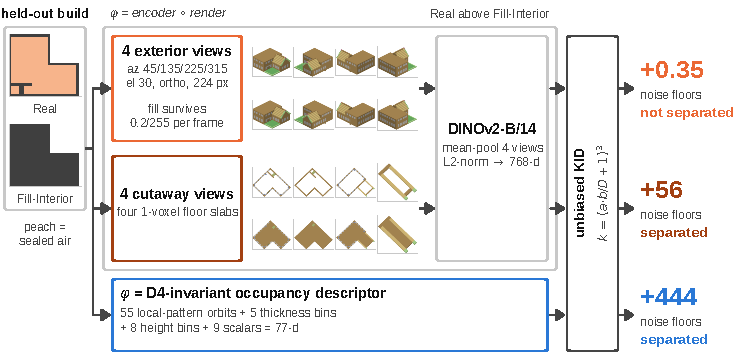
\includegraphics[width=0.95\linewidth]{figures/fig_pipeline}
\caption{\textbf{One estimator, three feature maps.} \mvkid{} and \vkid{} are the
same unbiased kernel distance of \maineq{eq:mmd} and differ only in $\phi$.
\emph{Row 1:} the render-and-embed path, where the structure reaches the statistic
as four images. \emph{Row 2:} the same renderer and the same encoder with cutaway
views, which recovers the signal. One renderer, one encoder, only the views
differ, and four other encoders and $8$ or $16$ views change nothing
(Table~\ref{tab:ablation}). \emph{Row 3:} the geometric path, which reads
occupancy directly and needs no renderer and no GPU. A noise floor is a run's own
real-vs-real spread and falls with $n$, so separations compare within a run: rows
$1$ and $3$ come from the $n{=}256$ leaderboard against $399$ reference builds,
and row $2$ from the view ablation at $n{=}256$ against $512$, where row $1$ scores $+0.2$. The
pixel residue in row $1$ is the mean over the $128$ exterior frames of the converse-probe run,
not one build. The sections at left are horizontal slices of one 3D-Craft build.}
\label{fig:pipeline}
\end{figure*}

\begin{figure*}[t]
\centering
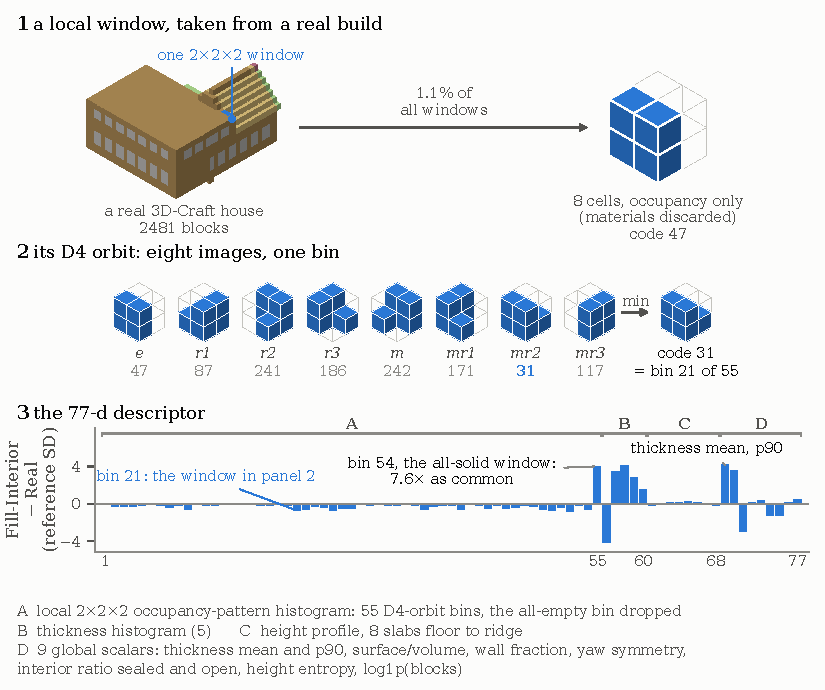
\includegraphics[width=0.92\linewidth]{figures/fig_descriptor}
\caption{\textbf{The geometric descriptor.} A $2\times2\times2$ occupancy
neighborhood, its orbit under the order-$8$ group of yaw rotations and an
$x$-mirror collapsing to one canonical bin, and the resulting feature vector with
the shift \solidify{} induces. The thickness histogram loses its one-block walls
and gains thick cores, and surface-to-volume with both interior ratios falls.
Filling every sealed interior moves this descriptor $202$ noise floors at
$n{=}128$, where the same builds move the render tier $0.14$.}
\label{fig:descriptor}
\end{figure*}

% =====================================================================
\section{Probes and Counting Interiors}
\label{app:interior}
% =====================================================================

\paragraph{Sealed air.} A cell is \emph{sealed} air when it is empty and not
$6$-connected through empty cells to the boundary of the build's bounding box.
\solidify{} fills exactly these cells with the build's most common material.
\hollow{} keeps a block only if one of its six faces borders air $6$-connected
to the outside, so it removes the solid behind the exterior shell, where \solidify{} fills
the sealed air behind it.

\paragraph{Counting rooms behind a doorway.} A naive enclosed-air count,
restricted to sealed air, counts a room with an open doorway as no room at all.
We additionally close the solid under a $26$-connected morphological closing
that seals openings up to two blocks wide and report the air that becomes
enclosed only then. Calibrated on a synthetic hollow cube with a $343$-cell room:
a $1{\times}1$, $1{\times}2$ or $2{\times}2$ doorway recovers all $343$ cells; a
$3{\times}3$ hole or a missing wall recovers $0$, correctly classifying an open
structure as having no room. On the same $200$ held-out houses the probe
statistics of \mainsec{sec:probes} are measured on, $\mathbf{6.0\%}$ have no
\emph{sealed} interior at all, and \emph{every one} of those twelve builds does
have a room reachable through a doorway. Per build, the sealed share of a
build's own interior volume has a median of $\mathbf{100\%}$ and a mean of
$\mathbf{85.5\%}$: most houses are fully sealed, and the rest lose a whole room
to an open door. Pooled over builds, apertures account for $\mathbf{25.6\%}$ of
total real interior volume, which is the margin by which a sealed-only counter
understates real houses. Every claim in the earlier literature that generated
builds ``have no interiors'' was made with that counter.

\paragraph{The dose axis.} \textsc{Partial-Fill} fills interior cells
\emph{inward from the walls}, nearest-first, which gives an exactly calibrated
dose (interior ratio $0.1175 \to 0.0941 \to 0.0708 \to 0.0475 \to 0.0242$).
Random speckle and largest-room-first filling were rejected, since the first
reads as noise and the second removes $71\%$ of the interior at a nominal $25\%$
dose. Fig.~\ref{fig:gallery} shows both probe directions on three builds.

\begin{figure}[t]
\centering
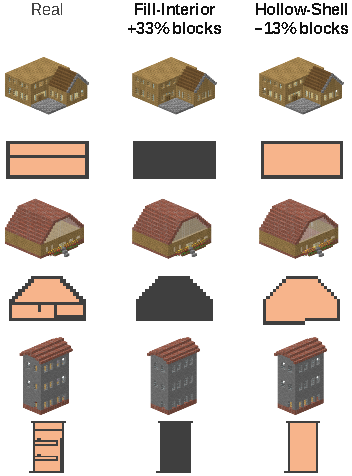
\includegraphics[width=0.8\linewidth]{figures/fig7_probe_gallery}
\caption{\textbf{Both directions of the corruption, on three held-out builds.}
\solidify{} adds a median $33\%$ blocks and \hollow{} removes a median $13\%$,
yet the views the metric is given are near-identical in every column. The
cross-sections show what changed, with sealed interior air in peach. In the converse-probe run at $n{=}256$, \mvkid{} places both within one noise
floor of real ($+0.21$ and $-0.02$); \vkid{} places them $402$ and $231$ away, against
$444.36$ and $265.4$ on the leaderboard's own floor.}
\label{fig:gallery}
\end{figure}

% =====================================================================
\section{Validation Gates}
\label{app:gates}
% =====================================================================

Every candidate metric is scored on rungs of known damage in units of its own
noise floor, and a metric that fails a gate is withheld from ranking
(\mainsec{sec:gates}). This section gives the render tier's ladder, the
procedural baselines, the provenance of each gate and the defects the gates
themselves had.

\subsection{The render ladder}

Table~\ref{tab:ladder-render} applies the gates to the render tier,
Table~\ref{tab:seven} gives the seven render-space statistics on the LEGO
ladder, and Fig.~\ref{fig:ladder} places both metrics on eight rungs of one run.
The per-metric ladder tables express a rung as its distance from the null
\emph{mean}, while the leaderboard expresses an arm as its distance from a
held-out \realheld{} \emph{draw}. On an exactly invariant rung the two
conventions differ by construction: the geometry metric's material-shuffle row
is $0$ exactly against the \realheld{} draw and $1.19$ against the null mean, so
the conventions must not be mixed within one comparison.

\begin{table*}[t]
\centering
\small
\caption{The render tier's metric-validation ladder (DINOv2-B, $4$ orthographic
views at $224$px, $n{=}64$). Columns are the probe rungs: real held-out, retype
$10\%$ of blocks (the rung the ordering gate uses for this tier), displace
$10\%$, delete $40\%$, material shuffle and a $90^\circ$ rotation; \textbf{sd}
is the metric's own noise floor. Gates are blocking, and \emph{only \textbf{KID}
and \textbf{MMD-RBF} pass}: PRDC coverage fails $n$-stability, and recall fails noise
ordering and invariance.
MMD-RBF is on its own scale and is reported to one decimal; the last row is the
biased estimator. The \emph{real} column scores a held-out draw against the reference, a
different null from the two disjoint halves of one real draw in \mainsec{sec:gates}, which
is why the unbiased KID does not read $0$ here.}
\label{tab:ladder-render}
\setlength{\tabcolsep}{3.5pt}
\begin{tabular}{lrrrrrrrl}
\toprule
       &      & retype   & displace & del.    & mat.    & rot.            & noise &      \\
metric & real & $10\%$ & $10\%$ & $40\%$ & shuffle & $90^\circ$ & floor & gate \\
\midrule
\textbf{KID} (unbiased) & \textbf{0.011} & \textbf{0.165} & \textbf{0.435} & \textbf{0.106} & \textbf{0.762} & \textbf{0.010} & \textbf{0.008} & \textbf{PASS} \\
\textbf{MMD-RBF} & \textbf{3.5} & \textbf{49.6} & \textbf{137.4} & \textbf{32.2} & \textbf{218.0} & \textbf{3.0} & \textbf{2.4} & \textbf{PASS} \\
$1-$recall & 0.137 & 0.331 & 0.899 & 0.371 & 0.790 & 0.105 & 0.028 & FAIL: noise ord., inv. \\
Fr\'echet distance & 0.107 & 0.157 & 0.250 & 0.147 & 0.373 & 0.106 & 0.005 & FAIL: $n$-stab. \\
$1-$coverage & 0.246 & 0.508 & 0.835 & 0.488 & 0.948 & 0.242 & 0.057 & FAIL: $n$-stab. \\
$1-$density & 0.000 & 0.247 & 0.637 & 0.166 & 0.897 & 0.000 & 0.073 & FAIL: noise ord. \\
$1-$precision & 0.125 & 0.234 & 0.234 & 0.109 & 0.641 & 0.125 & 0.036 & FAIL: noise ord. \\
biased MMD estimator & 0.079 & 0.468 & 1.148 & 0.317 & 1.987 & 0.075 & 0.021 & FAIL: $n$-stab. \\
\bottomrule
\end{tabular}
\end{table*}

\begin{table}[t]
\centering
\small
\caption{The render-tier ladder on the LEGO domain (StableText2Brick, DINOv2-B,
$4$ views, $n{=}128$), each statistic in its own noise floors, measured from the
floor's mean rather than from a held-out draw, so these values are not directly comparable
with Table~\ref{tab:ablation}'s or with \maintab{tab:lego}, where the same probe reads
$-0.09$ on \mvkid{} at $n{=}253$. \textbf{All seven miss \solidify{} and resolve
every other corruption.}}
\label{tab:seven}
\resizebox{\linewidth}{!}{%
\begin{tabular}{lrrr}
\toprule
statistic & \solidify{} & $20\%$ deleted & \matshuffle{} \\
\midrule
KID & $\mathbf{2.0}$ & 12.3 & 132.3 \\
MMD-RBF & $\mathbf{2.1}$ & 13.9 & 148.8 \\
Fr\'echet distance & $\mathbf{0.5}$ & 10.8 & 72.4 \\
$1-$coverage & $\mathbf{0.2}$ & 7.7 & 19.8 \\
$1-$density & $\mathbf{0.1}$ & 7.2 & 14.0 \\
$1-$precision & $\mathbf{-0.4}$ & 9.0 & 28.0 \\
$1-$recall & $\mathbf{0.4}$ & 1.4 & 30.7 \\
\bottomrule
\end{tabular}}
\end{table}

\begin{figure}[t]
\centering
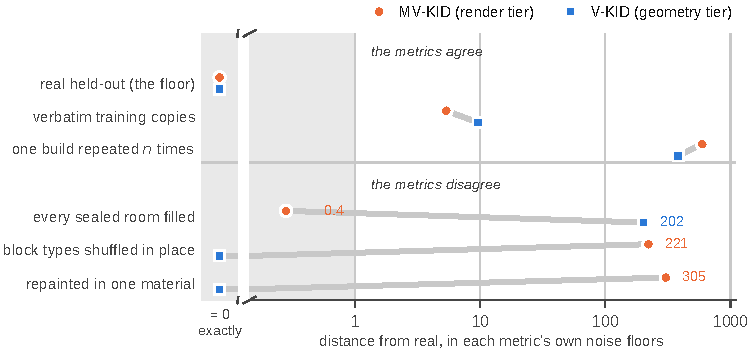
\includegraphics[width=\linewidth]{figures/fig10_ladder}
\caption{\textbf{Two metrics, one run, eight rungs of known damage.} Each rung's distance
from held-out real, in that metric's own noise floors ($n{=}128$, symlog). The geometric metric's two material rungs are bit-identical to real, not merely small,
so they sit in a separate gutter. The band marks one noise floor; per-statistic numbers are in
Table~\ref{tab:seven}.}
\label{fig:ladder}
\end{figure}

\subsection{Procedural baselines}

\begin{table*}[t]
\centering
\small
\caption{Procedural baselines, with real held-out data for reference.
\gabled{} is the bar that matters: what a competent afternoon of hand-written
rules produces. \patchstitch{} is an attack, not a baseline. Every cell is a
per-build mean over $n{=}128$ builds per baseline; the real row is all $399$
held-out test builds. \textbf{Interior is reported twice}, because the two
counters answer different questions (Sec.~\ref{app:interior}):
\emph{sealed} is air unreachable from the bounding box, \emph{open} additionally
credits rooms reachable only through a door or window. The distinction is not
cosmetic: \gabled{} has a doorway, so it scores $0.000$ sealed and $0.562$
open.}
\label{tab:baselines}
\setlength{\tabcolsep}{4pt}
\begin{tabular}{llrrrrr}
\toprule
& & & & \multicolumn{2}{c}{interior} & \\
\cmidrule(lr){5-6}
baseline & what it is & blocks & wall frac & sealed & open & LCC \\
\midrule
\randomvox{} & random voxels at real density & 1383 & 0.049 & 0.002 & 0.003 & 0.406 \\
\hollowbox{} & hollow box, floor, walls, flat roof & 1345 & 1.000 & 0.609 & 0.609 & 1.000 \\
\patchstitch{} & $8^3$ patches from \emph{different} builds & 1405 & 0.624 & 0.003 & 0.009 & 0.866 \\
\gabled{} & box, pitched roof, door, windows & 1139 & 0.969 & 0.000 & 0.562 & 1.000 \\
\copynoise{} & a training build, $10\%$ displaced & 1057 & 0.454 & 0.002 & 0.055 & 0.967 \\
\midrule
\textbf{real} & held-out test split & 924 & 0.745 & 0.114 & 0.129 & 0.978 \\
\bottomrule
\end{tabular}
\end{table*}

\paragraph{Why coherence is reported as distance to real.} Two rows at the extremes of
\maintab{tab:leaderboard} show why the suite reports more than its two realism pillars.
An arm of \emph{verbatim copies of the training set} scores $0.012$ raw \mvkid{}, third of
sixteen arms, behind only held-out real data and \solidify{}, and only the novelty columns
catch it: nearest-neighbor IoU $1.000$, duplicate rate $1.000$ and a retrieval percentile
of $0.000$ against a real held-out floor of $0.507$. At the other end of the scale the
procedural baselines are \emph{too} hollow, with aperture-aware interior ratios of $0.61$
(\hollowbox{}) and $0.56$ (\gabled{}) against a real $0.13$. A coherence measure read as
``higher is better'' would therefore rank a hollow box above a house, which is why every
coherence measure is reported as distance to real.

% Source: outputs/run_20261106_193109_gate_provenance (notes §84, results T107).
\subsection{Where the gates come from, and whether they favour \vkid{}}
\label{app:gateprov}

\vkid{} and the gates that admit it come from one project, so the gates need
evidence that they were not shaped around it. We give three kinds: each gate's
prior use, when each threshold was set, and the verdicts of
Table~\ref{tab:headtohead} under alternative thresholds.

\paragraph{Prior use.} Table~\ref{tab:gateprov} maps each gate to earlier work
that states the same criterion. Ordering under graded corruption is the test
FID was introduced with \citep{heusel2017fid}, repeated for KID
\citep{binkowski2018kid} and made a rank-correlation criterion for graph
metrics \citep{obray2022graphmetrics,thompson2022evaluation}. Invariance to
quality-preserving transforms is a stated desideratum
\citep{borji2019prosandcons,borji2022newdevelopments}, and FID's violations of
it are documented \citep{kynkaanniemi2023imagenet,parmar2022aliased}. A metric
that cannot recognise two samples of one distribution fails the test
\citet{naeem2020prdc} apply to precision and recall, and sample-size bias is
the defect \citet{binkowski2018kid}, \citet{chong2020unbiasedfid} and
\citet{jayasumana2024cmmd} identify in FID. The memorization gates follow the
held-out-referenced data-copying test of \citet{meehan2020datacopying}, and the
within-set twin gate follows the approximate-copy diversity test of
\citet{jiralerspong2023fld}. Text-metric checklists apply the same
directional and invariance tests \citep{ribeiro2020checklist,sai2021perturbation}.
What we change is the use: a failing metric is withheld from ranking rather
than reported with a caveat. \citet{obray2022graphmetrics} use graded perturbations
to select metric hyperparameters, never to disqualify a metric, and without an
invariance or sample-size test; \citet{borji2019prosandcons} list the desiderata
without running them as a gate. The one prior meta-evaluation of metrics in this
domain, \citet{herve2021pcgmetrics}, correlates eighteen procedural-content metrics
with GDMC jury scores, the route a human-validated version of this suite would take.

\begin{table}[h]
\centering
\small
\setlength{\tabcolsep}{3pt}
\begin{tabular}{lp{0.62\linewidth}}
\toprule
gate & prior statement of the criterion \\
\midrule
G1, G2 ordering & \citet{heusel2017fid,binkowski2018kid,xu2018empirical,obray2022graphmetrics,thompson2022evaluation,jayasumana2024cmmd,jiralerspong2023fld} \\
G6 invariance & \citet{borji2019prosandcons,borji2022newdevelopments,kynkaanniemi2023imagenet,parmar2022aliased,ribeiro2020checklist} \\
G7 self-consistency & \citet{naeem2020prdc,binkowski2018kid,lopezpaz2017c2st,yang2019pointflow} \\
G8 $n$-stability & \citet{binkowski2018kid,chong2020unbiasedfid,jayasumana2024cmmd,jiralerspong2023fld,thompson2022evaluation} \\
memorization & \citet{meehan2020datacopying,alaa2022faithful,jiralerspong2023fld,stein2023exposing,somepalli2023replication} \\
diversity, twins & \citet{xu2018empirical,naeem2020prdc,jiralerspong2023fld} \\
\bottomrule
\end{tabular}
\caption{\textbf{Each gate restates a published criterion.}}
\label{tab:gateprov}
\end{table}

\paragraph{When the thresholds were set.} The ordering, invariance, self-consistency and $n$-stability thresholds were committed and validated on render
metrics four weeks before the first voxel-descriptor metric existed, and the gate code,
with the $77$-dimensional descriptor, has been unchanged for $58$ days before the
head-to-head of Sec.~\ref{app:headtohead} ran. The only later change to the gates is the
pair of denominator corrections of Sec.~\ref{app:defects}, which apply to every metric;
the twin gate reuses the duplicate gate's rule.

\paragraph{Verdicts under other thresholds.} We recompute every gate of
Table~\ref{tab:headtohead} from the stored scores and, for \vkid{}, occupancy KID
and the six IoU rows, from a rerun that reproduces the table to $2\times10^{-6}$
and also records each null mean and drift. Each threshold moves over a range
around its value: ordering tolerance from $-1$ (each step must rise by one
floor) to $+2$ (a step may fall by two), the invariance bar from $0.5$ to $5$
floors, and the self-consistency and $n$-stability bars from $1$ to $5$.
\begin{itemize}
\item At every ordering tolerance $\le 0$ and every invariance bar, with the
  other two bars at their values, \vkid{} is the only row that passes
  (Fig.~\ref{fig:gatesweep}).
\item \vkid{} passes in all $360$ of the $480$ joint settings with a
  self-consistency bar of at least $2$ floors. A bar of $1$ floor rejects every
  row, \vkid{} included, as a single draw lies within one floor of its mean only
  about two thirds of the time.
\item Its margins are wide: the smallest ordering step is $7.5$ floors,
  invariance holds exactly, the self-consistency deviation is $1.2$ floors and the
  drift is $0.4$ standard errors.
\item The rows a looser threshold admits are those whose failure is a tie
  rather than an inversion. Allowing a step to fall by half a floor admits
  1-NNA on IoU and EMD, which separate \solidify{} by $2.7$ and $1.6$ floors;
  adding an invariance bar of $2$ floors admits occupancy KID ($48.4$). No
  threshold admits an encoder as a geometry metric, since \matshuffle{} and
  \monochrome{} move them by $63$ to $106$ floors, nor IoU nearest-neighbour MMD,
  whose $n$-drift is $34$ to $36$ standard errors.
\end{itemize}
The same holds for disqualification. Across novelty bars of $2$, $3$ and $5$
spreads and floors of half, one and two times their values, both positive
controls, Dream-Cubed and the hollow-box baseline are disqualified in all nine
settings. Only the loosest corner readmits an arm, the gabled-house baseline, and tightening to $2$ spreads first
disqualifies our own autoregressive arms on DINO nearest-neighbour percentile.

\begin{figure}[h]
\centering
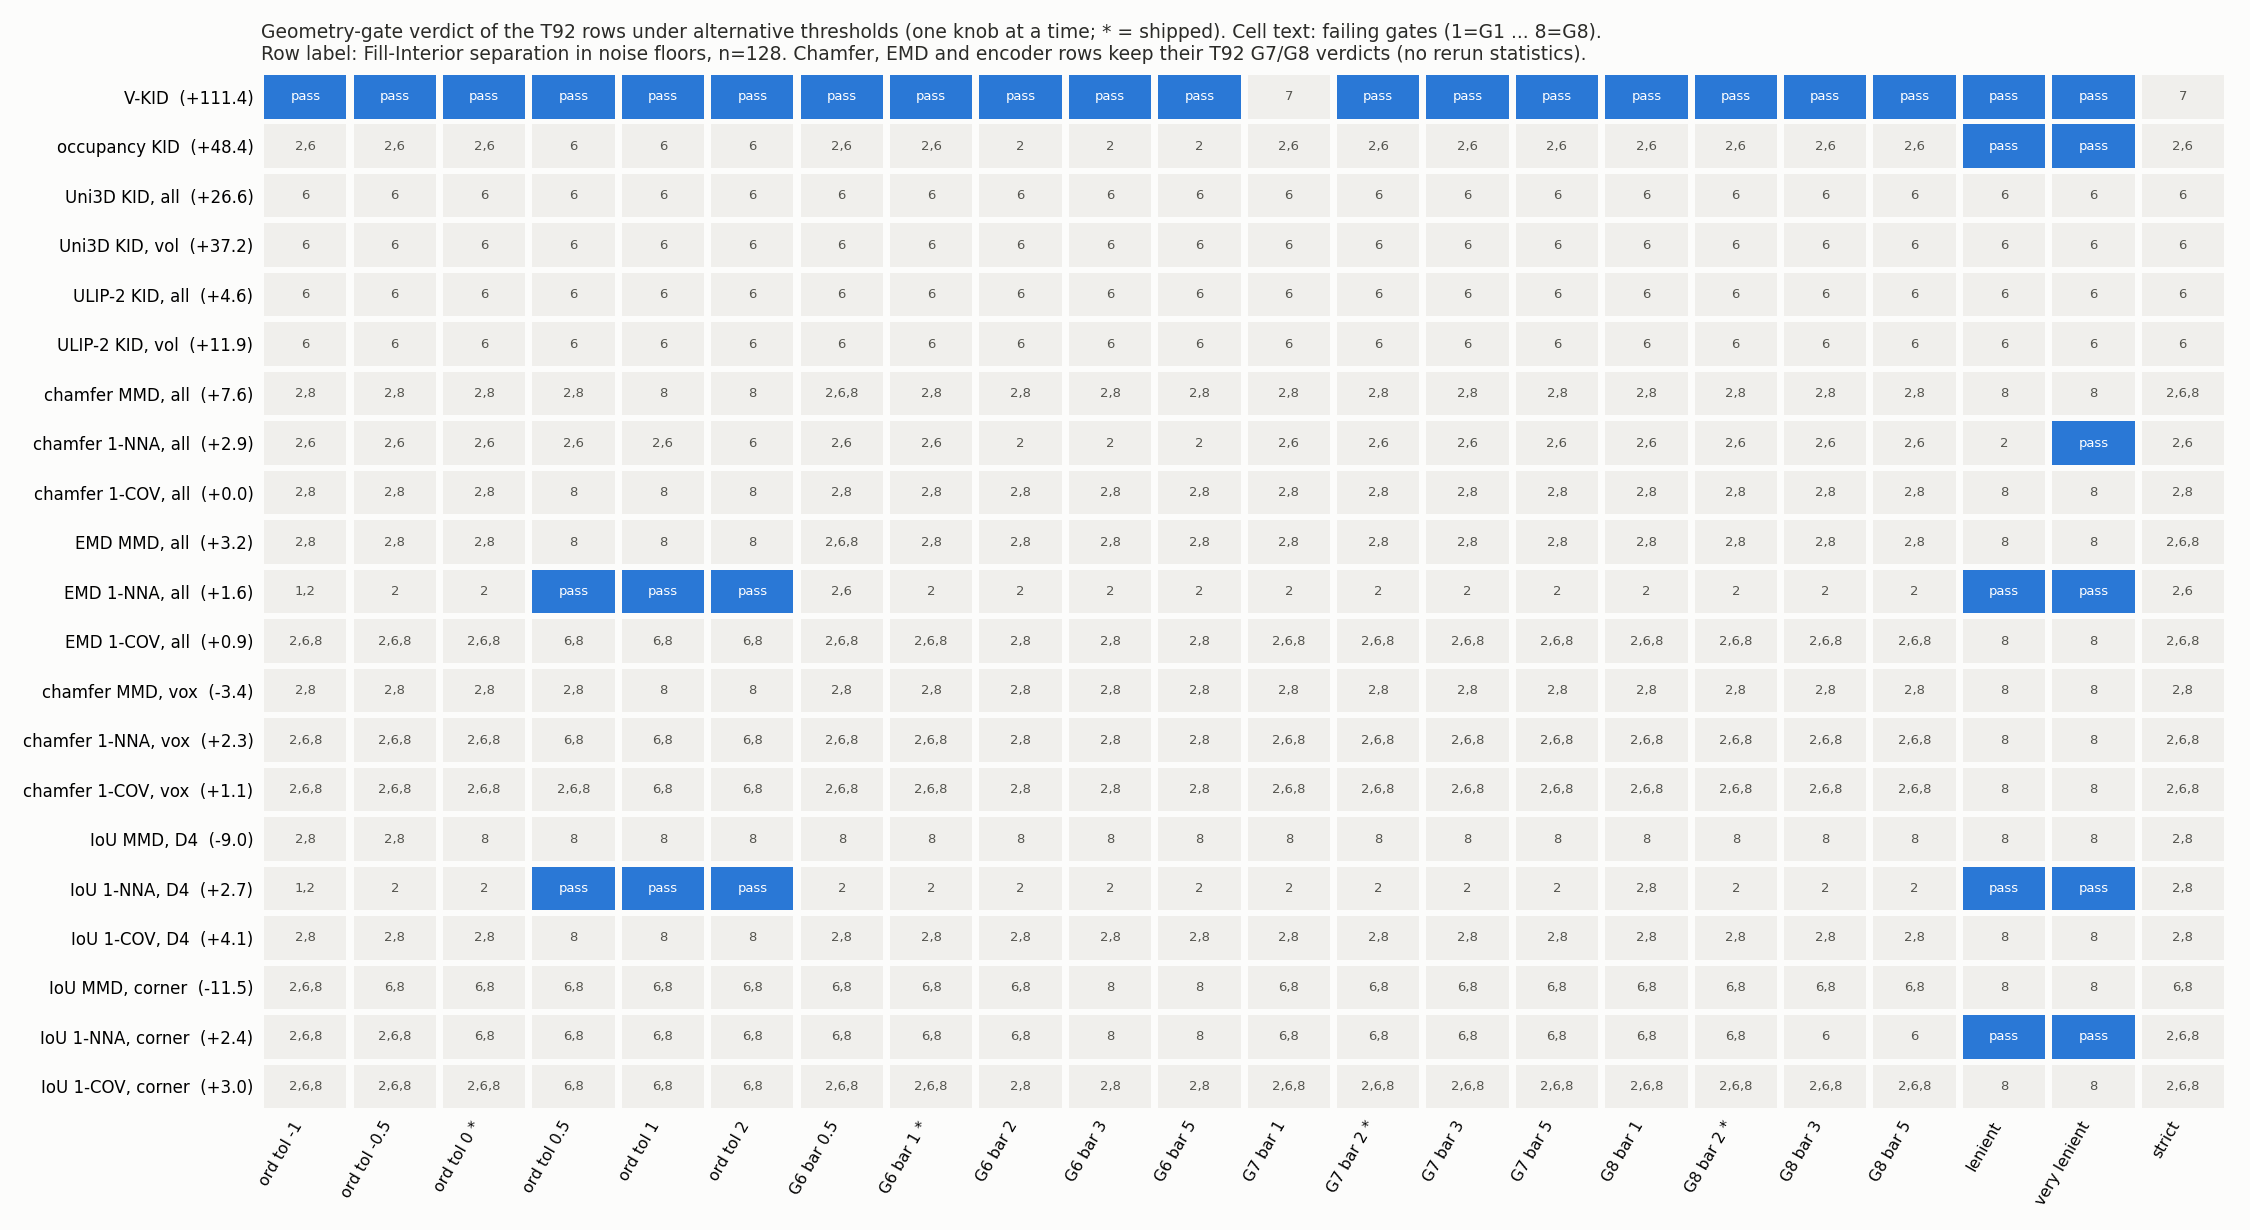
\includegraphics[width=\linewidth]{figures/gate_sweep.png}
\caption{\textbf{Gate verdicts under alternative thresholds.} Rows of
Table~\ref{tab:headtohead} with their \solidify{} separation; columns move one
threshold at a time ($*$ marks the value used) or all four together. Blue:
passes every gate on the geometry rungs. Text: the gates that fail.}
\label{fig:gatesweep}
\end{figure}


\subsection{Auditing the gates}
\label{app:defects}

A gate needs auditing like any other measurement, and ours had two denominator
defects and one fail-open renderer. The noise floor, the unit every gate is
stated in, was first estimated from subsamples of a pool that excluded the probe
set and carried no finite-population factor; corrected, a metric that separates
\solidify{} at $67$ s.d.\ passes the self-consistency gate it had failed. The
$n$-stability gate first tested a difference of means against the spread of a
single draw, larger by $\sqrt{\text{reps}}$; against the standard error of the
difference, the biased estimator's $1/n$ decay is rejected at $14.8$ standard
errors. Separately, the renderer once substituted a blank frame for any
rendering exception, so a library mismatch made every arm score KID
$=-4\times 10^{-13}$, better than real. It now raises past a $2\%$ failure rate,
and the repaired library reproduced the stored render canary bit-for-bit, so no
recorded number is affected.

% =====================================================================
\section{Aggregation and Statistical Reading}
\label{app:stats}
% =====================================================================

\subsection{What \blockscore{}'s maximum is}
\label{app:blockscore}

%TL;DR of paragraph: a max over k pillars has a positive null, so a fresh real arm scores about 1.1 rather than 0.
\blockscore{} is the maximum of five pillar scores, and a maximum of several
mean-zero quantities is not itself mean-zero. The control arm reads exactly
$0.00$ on every pillar because it \emph{is} the arm the calibration is taken
from: $(v_p - v_p)/\mathrm{sd}_p = 0$ identically, with zero variance. That is
an identity, not a measurement, and \maintab{tab:leaderboard} labels it as
such. A \emph{fresh} real arm, drawn from the same distribution but not used to
calibrate, scores $\mathbb{E}[\blockscore] = 1.08$ with standard deviation
$0.89$, right-skewed ($+0.89$), and a $95$th percentile of $2.8$. Read
\blockscore{} against that null rather than against zero: a value of $15$ is not
``$15$ standard deviations'' but ``far outside a null whose upper tail is under
$3$''. The inflation is about one noise floor, against a smallest score
of $229.29$ on the leaderboard, so it changes no ordering and no conclusion in this paper. A
future suite comparing arms that sit within a few floors of real would need to
subtract it.

%TL;DR of paragraph: three pillars are in real noise floors and two are in a coarser unit, so the max is a veto over three.
The five pillars are not in one unit. Appearance, geometry and palette are
divided by a genuine sampling noise floor, and we verify this: their declared
units match the spread of fresh real draws to within $7\%$ ($0.93$, $1.03$ and
$1.05$ of the measured value). The coherence and geometry-scalar pillars are
divided by a per-build robust spread of the reference, an effect size measuring how
far apart two distributions are in units of how much individual builds differ.
Measurement puts that unit $29\times$ and $52\times$ coarser than those
pillars' own sampling noise. A structure pillar would therefore have to move
some $4{,}800$ of its actual noise floors to veto a live pillar sitting at
$+166$, and on our card none ever does. We state this as a limitation of the
current calibration rather than a property of the aggregation rule: the maximum
is the right rule, and two of the five inputs are quoted in a unit that makes
them diagnostics rather than vetoes.

%TL;DR of paragraph: the number is only interpretable beside the name of the pillar that produced it.
Because the winning pillar's unit is what the number is in, \blockscore{} is
uninterpretable without the pillar that produced it, which is why every
leaderboard we print carries a \emph{worst pillar} column. It is also not
convertible to a $p$-value: the null is max-shaped and skewed, so the usual
normal reading does not apply.

\subsection{The noise-floor unit depends on $n$}
\label{app:nscale}

Separations throughout this paper are quoted in \emph{noise floors}: the
standard deviation of repeated real-versus-reference draws at the same sample
size. That unit makes two metrics with incommensurable raw scales comparable
within a run, which is why we use it. It is not scale-free across runs,
and we state the dependence explicitly because it is easy to misread.
Measured on the identical corruption at two sample sizes in the dose run ($399$ reference
builds, its own $48$-draw floor):

\begin{center}
\small
\resizebox{\linewidth}{!}{%
\begin{tabular}{lrrrrrr}
\toprule
metric & sd $n{=}64$ & sd $n{=}128$ & ratio & sep $n{=}64$ & sep $n{=}128$ & ratio \\
\midrule
\vkid{} & 0.1732 & 0.0848 & \textbf{0.49} & 132.9 & 286.7 & \textbf{2.16} \\
\mvkid{} & 0.00438 & 0.00316 & 0.72 & 0.48 & 0.34 & 0.71 \\
\bottomrule
\end{tabular}}
\end{center}

The noise floor of the geometric metric halves when $n$ doubles, the $1/n$ decay
expected of a degenerate U-statistic under the null, while the
population effect is fixed. A separation in noise floors therefore grows
\emph{linearly} in $n$, and a figure such as ``$202$'' means ``$202$ at
$n{=}128$''. The $n{=}256$ leaderboard measures the same probe against the same
reference at $444.36$, a factor of $2.2$ (Sec.~\ref{app:n256}). Separations are
therefore only comparable across runs at equal $n$, which is why our protocol
pins it, and regenerating every arm at a larger $n$ leaves the \emph{ordering} of
arms intact while roughly doubling every magnitude. \mvkid{} scales less cleanly
($0.72$ rather than $0.49$) because its separation is a ratio of two quantities
that are both near zero, and the render row should be read as
``indistinguishable'', not as a number.

\paragraph{The unit is itself estimated.} The floor comes from $48$
real-versus-reference draws and carries a relative standard error near
$1/\sqrt{2 \cdot 47} \approx 10\%$, so a separation should be read to one or two
significant figures with its run named. We quote $202$ because it is the
protocol run's value; a sweep over twelve seeds places it between $185$ and
$274$. The dose run above draws its own floor against the same reference ($0.0848$ at
$n{=}128$ against the protocol run's $0.110$) and reads the same probe at $286.7$, and the
validation ladder, which scores against a $248$-build subset and measures from the null
mean, reads $111.4$ (Table~\ref{tab:headtohead}).

\paragraph{The linear-in-$n$ rule holds at fixed reference size.} The
doubling above, $202$ at $n{=}128$ to $444$ at $n{=}256$, assumes the reference
pool is unchanged. Our view-protocol ablation measures the same probe on the
same corpus and split at $n{=}256$ and reads $120.8$, not $400$, because it
scores against $512$ reference builds rather than $399$ and its floor
($0.188$) is consequently \emph{larger} than the $n{=}128$ floor rather than
half of it. The rule describes how a separation moves when $n$ grows within one
protocol; it does not survive a change of reference, which is why every number
in this paper is reported with its run.

\subsection{The $n{=}256$ leaderboard and the $n{=}128$ protocol run}
\label{app:n256}

The leaderboard of \maintab{tab:leaderboard} reruns the protocol run's board at the
protocol's own $n{=}256$, with the same reference, split, $77$-dimensional
descriptor and seed. The generator arms were extended from $128$ to $256$
samples from the same checkpoints and sampling stream, so the first $128$
samples of every arm are byte-identical to the protocol run's.

\begin{table}[h]
\centering
\small
\setlength{\tabcolsep}{3pt}
\caption{\blockscore{} and rank at $n{=}128$ (protocol run) and $n{=}256$ (leaderboard).
Raw kernel distances barely move; the noise floor roughly halves, so every \blockscore{} roughly
doubles. Ranks are the leaderboard's own; ties as in \maintab{tab:leaderboard}. The
$n{=}256$ \blockscore{} of an arm the within-set near-twin gate disqualifies (DQ) is the
maximum pillar it would have scored (Sec.~\ref{app:dreamcubed}); the gate postdates the
protocol run, so the $n{=}128$ column is ungated.}
\label{tab:n256}
\begin{tabular}{lrrrr}
\toprule
arm & \multicolumn{2}{c}{\blockscore{}} & \multicolumn{2}{c}{rank} \\
\cmidrule(lr){2-3}\cmidrule(lr){4-5}
 & $n{=}128$ & $n{=}256$ & $128$ & $256$ \\
\midrule
Dream-Cubed              & ---      & $165.71$ & ---  & DQ \\
\voxar{} (contaminated)  & $106.87$ & $229.29$ & 2    & 2 \\
\voxar{} (clean)         & $136.73$ & $285.22$ & 3    & 3 \\
\voxarun{} (clean)       & DQ       & $345.10$ & DQ   & 4 \\
\matshuffle{}            & $231.52$ & $422.43$ & 7    & 5--7 \\
\patchstitch{}           & $246.15$ & $431.70$ & 8    & 5--7 \\
\solidify{}              & $201.80$ & $444.36$ & 6    & 5--7 \\
\monochrome{}            & $297.95$ & $535.36$ & 9    & 8 \\
\copynoise{}             & $302.73$ & $619.13$ & 11   & 9 \\
\gabled{}                & $300.15$ & $620.98$ & 10   & DQ \\
\hollowbox{}             & $476.22$ & $864.00$ & 12   & DQ \\
\randomvox{}             & $603.09$ & $1087.06$ & 13  & 10 \\
\bottomrule
\end{tabular}
\end{table}

Table~\ref{tab:n256} sets the two boards side by side. The noise floor roughly halves at
$n{=}256$ ($0.110\to0.053$ for \vkid{}, $0.00289\to0.00161$ for \mvkid{}) while the raw
distances hold (\voxar{} clean: \vkid{} $14.90\to15.06$, \mvkid{} $0.245\to0.254$), so
separations double and only ranks and ratios carry across. Three changes go beyond the
doubling. \voxarun{}'s memorization gate was marginal at $n{=}128$, $+3.0$ spreads against
a bar of $3.0$; at $n{=}256$ it reads $+2.1$ and the arm ranks fourth. The within-set
near-twin gate disqualifies Dream-Cubed, \gabled{} and \hollowbox{}
(Sec.~\ref{app:dreamcubed}). Among the controls, \matshuffle{}, \patchstitch{} and
\solidify{} become a three-way tie (adjacent flip probabilities $0.20$ and $0.21$). The rank intervals are $95\%$ intervals over
$1{,}000$ replicates that subsample $80\%$ of every arm and share one reference subsample
per replicate; a pair is a tie when its order flips in at least $5\%$ of replicates.
% =====================================================================
% BLOCK C. Noise-floor audit.
% REPLACES the last four sentences of \subsection{The $n{=}256$ leaderboard and
% the $n{=}128$ protocol run} (\label{app:n256}), from "The noise floor at
% $n{=}256$ is estimated from $256$ of the $399$ test builds per draw" to
% "The ranks do not depend on it." The rank-interval sentences before them stay.
% Also EXTENDS \paragraph{The unit is itself estimated.} in app:nscale: no edit
% needed there, the last two sentences below cite its 10% figure.
% =====================================================================
\paragraph{Calibrating the finite-population correction.} The floor at $n{=}256$ draws
$256$ of the $399$ test builds per replicate and divides the spread of those overlapping
draws by $\sqrt{1-n/N}$. For a degenerate U-statistic the leading variance term carries
$(1-f)^2$ rather than $(1-f)$, which would make this correction too small, but the pool's own
kernel matrix adds a first-order term of order $\zeta_2/N$ that more than offsets it. We
measure the net effect against non-overlapping draws: a reference of $399$ and a population
of $1{,}464$ real builds, both drawn from the training split so that the statistic sits in the
same near-degenerate regime, with the true spread read off disjoint $n$-sets of the
population. The true spread is $0.88$ to $0.95$ of the bench floor at $n{=}256$ and $0.89$ to
$0.93$ at $n{=}128$, for both metrics, so the floor is slightly conservative; a $(1-f)$
correction would overstate it by a factor near $1.8$. On the leaderboard's own pool an
unbiased Hoeffding estimate, accurate to $5\%$ in the simulation, puts the stored \vkid{}
floor $11\%$ above the true one and the stored \mvkid{} floor $2.5\%$ below it. The larger
term is the Monte-Carlo error of Sec.~\ref{app:nscale}: $48$ draws pin the \vkid{} floor at
$n{=}256$ only to $[0.043, 0.067]$ at $95\%$, which is why two runs scoring the same raw
distance against two $48$-draw floors can read \matshuffle{} at $+422$ and at $+346$. We keep
each run's stored floor; under the corrected floor no gate verdict of \vkid{} or \mvkid{}
changes and no ranking changes.

\subsection{The head-to-head test}
\label{app:significance}

%TL;DR of paragraph: pairs are compared by an exact label-permutation test against a fixed reference, which is calibrated in both regimes of the statistic.
Arm pairs are compared with an exact label-permutation test: pool the two arms,
re-split at the observed sizes, and recompute the difference of kernel distances
against the same fixed reference, with Holm correction \citep{holm1979simple}
over the family of pairs. A resampling estimate of the standard error does not
work here, because the difference is a degenerate U-statistic when both arms
match the reference and a non-degenerate one when they do not, so no single
rescale is correct. The permutation null tracks a Monte-Carlo ground truth within
$5\%$ in both regimes and its type-I error is nominal at both levels. An earlier
subsampling test rejected $3.4\times$ too often on matched nulls and $7.2\times$
on mismatched ones, and a floored bootstrap $p$-value earlier made every pair
unseparable after Holm; both are replaced.

%TL;DR of paragraph: recomputing the run of record leaves both null results intact and costs two positive separations.
Recomputing the run of record changes only claims of separation, which is the
expected direction: a test that rejects too easily can manufacture a difference
but never a tie. Both of our null results hold and strengthen: \solidify{}
remains unseparated from held-out real ($p$ from $0.61$ to $0.77$), and the clean
retrain remains unseparated from the language-model baseline ($0.89$ to $0.93$).
Two positive separations do not survive: \traincopy{} against held-out real falls
to the $\alpha{=}0.05$ boundary, and the contaminated arm separates from one
language-model baseline but not the other. We report the blindness result by
magnitude for this reason, and the case study's conclusion, that the contaminated
arm's apparent advantage does not survive a clean split, is
unaffected, since it rests on a within-architecture comparison.

% =====================================================================
% BLOCK B. Detection-n and equivalence.
% EXTENDS \subsection{The head-to-head test} (\label{app:significance}): append
% after its second paragraph ("Recomputing the run of record ..."). Nothing in
% that subsection is replaced; its p from 0.61 to 0.77 is the n=128 protocol
% run, the 0.87 below is the n=256 leaderboard draw.
% Figure file: drafts_20261109/fig_detection.pdf -> figures/fig_detection.pdf
% =====================================================================
\paragraph{Non-detection, and equivalence.} Every probe is built from the same builds as the
real arm it is compared with. The label-permutation test treats the two arms as independent,
which is exact under its null but discards the pairing, so on a probe it is conservative:
\solidify{} against real reads $p{=}0.87$ at $n{=}256$. A paired test that swaps labels
within each build and its probe reads $p{=}0.055$ for the same $+0.35$ floors, and $0.82$ for
\hollow{}. Across $n$ from $8$ to $256$ the paired test never reaches $80\%$ power on either
interior probe under \mvkid{} (at most $0.20$), while \vkid{} detects both at $n{=}8$
(Fig.~\ref{fig:detection}). Non-rejection is not equivalence, so we also test equivalence
against a margin fixed in advance, two noise floors, with two one-sided tests whose standard
error is that of a fresh draw of $256$ builds and of the reference, from the Hoeffding
decomposition of the paired difference. \solidify{} reads $+0.35$ floors with $90\%$
interval $[-0.28, +0.98]$ and \hollow{} $+0.04$ with $[-0.25, +0.33]$, both equivalent to real
($p{<}0.001$); the same holds for a margin of $0.05$ in effect size ($\pm 2.7$ floors). Under
\vkid{} neither is equivalent, at $444$ and $265$ floors.

\begin{figure*}[t]
\centering
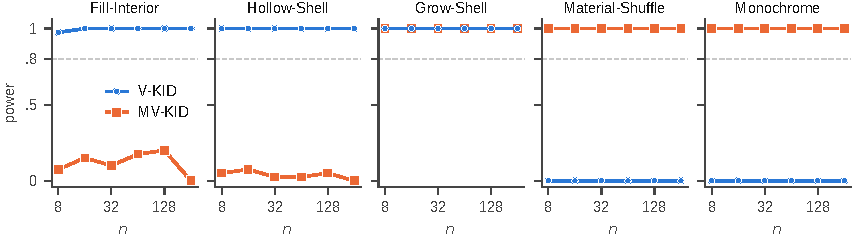
\includegraphics[width=\linewidth]{figures/fig_detection}
\caption{\textbf{Detection as a function of $n$.} Power of the paired permutation test
($\alpha{=}0.05$, $999$ permutations) of each probe against its own source builds, over $40$
random subsets per $n$ below $256$ and the full set at $n{=}256$; dashed line, $80\%$.
\vkid{} detects \solidify{}, \hollow{} and \growshell{} at $n{=}8$. \mvkid{} detects
\growshell{}, \matshuffle{} and \monochrome{} at $n{=}8$ and never reaches $80\%$ power on
\solidify{} or \hollow{}.}
\label{fig:detection}
\end{figure*}

\subsection{Reading a squared statistic over a population of prompts}
\label{app:failrate}

How a metric's value is \emph{read} is a separate issue from what it can see.
Because KID and MMD are squared, an arm that fails on a quarter of its builds
scores only $6.0\%$ of the way to fully bad, where a reader assuming
proportionality would infer a quarter of the damage. For a squared-MMD
statistic the response to a mixture is quadratic,
\begin{equation}
\mathrm{MMD}^2\!\left(\alpha P + (1-\alpha)Q,\; P\right)
  = (1-\alpha)^2\,\mathrm{MMD}^2(Q, P),
\label{eq:mixture}
\end{equation}
a one-line consequence of the linearity of the mean embedding.
\citet{binkowski2018kid} state this identity in their Appendix B.2, and both they and
\citet{heusel2017fid} plot their metrics against a contamination fraction. We add the
reporting recommendation it implies: report $\mathrm{MMD} = \sqrt{\mathrm{MMD}^2}$, which
is \emph{linear} in the contaminated fraction and free to compute. The identity holds for
squared integral probability metrics such as KID and MMD. It does not hold for
Fr\'echet distance, which \citet{binkowski2018kid} show is not polynomial in $\alpha$,
so we derive the correction for KID only.

%TL;DR of paragraph: the measured exponent, the compression it causes, and what the square root recovers.
Measured on a mixture ladder whose bad pool is \randomvox{} at $n{=}128$, the best-fit
exponent of \mvkid{} is $\mathbf{2.05}$ against the identity's $2$. An arm failing on a
quarter of its builds scores $6.0\%$ of the way to fully bad ($0.105$ against $1.740$).
Reporting $\sqrt{\mathrm{KID}}/\sqrt{\mathrm{KID}_{\text{worst}}}$ recovers the true bad
fraction to a mean absolute error of $\mathbf{0.013}$ (\mvkid{}) and $\mathbf{0.020}$
(\vkid{}), against $0.128$ and $0.131$ for the raw values.

%TL;DR of paragraph: the estimator is unbiased for the square, not its root, so the readout is a diagnostic rather than a ranked quantity.
One caution on the readout. The identity holds for the population quantity, while we
report an unbiased estimator of $\mathrm{MMD}^2$, which can be negative and whose square
root is therefore biased downward by Jensen's inequality, worst where the statistic is
small relative to its own standard error. We report the square root as a diagnostic for
reading a failure rate, never as the ranked quantity.

% =====================================================================
% =====================================================================
% BLOCK A. Effect size.
% EXTENDS \subsection{Reading a squared statistic over a population of prompts}
% (\label{app:failrate}): append after its last paragraph ("One caution on the
% readout ..."). Nothing in that subsection is replaced.
% =====================================================================
\paragraph{An effect size for comparing metrics.} A separation in noise floors is a test
statistic: it grows linearly in $n$ (Sec.~\ref{app:nscale}) and at a different rate per
metric, so a ratio of two metrics' separations is not a ratio of what they see. The readout
above gives a quantity that does not grow with $n$,
$e = \sqrt{\mathrm{MMD}^2_{\text{arm}}}\,/\,\sqrt{\mathrm{MMD}^2_{\randomvox{}}}$ under the
same metric, which reads $0$ for real data and $1$ for the anchor whatever the metric.
Table~\ref{tab:effect} gives it for every probe at $n{=}256$. The two interior probes sit at
$0.03$ and $0.02$ of the anchor on appearance, inside the $95$th percentile of fresh real
draws ($0.031$), and at $0.78$ and $0.60$ on geometry. \matshuffle{} and \monochrome{} are
the converse. \patchstitch{} sits as far from real on geometry as on appearance, so its
near-real local statistics buy it no geometric advantage. Read between a probe and its own
source builds, the render features of \solidify{} do move, by $0.018$ $[0.014, 0.024]$ of the
anchor against a paired null of $0.005$: that is the glass leak of Sec.~\ref{app:hull}, $44$
times smaller than \vkid{}'s $0.80$ on the same pairs.

\begin{table}[h]
\centering
\small
\setlength{\tabcolsep}{3pt}
\caption{\textbf{Effect size} $e$, $\sqrt{\mathrm{MMD}^2}$ over that of \randomvox{} under
the same metric, $n{=}256$ against the $399$-build reference, with half-sampling $95\%$
intervals. The $95$th percentile of fresh real draws is $0.031$ (\mvkid{}) and $0$
(\vkid{}). BrickGPT is scored on the LEGO suite, where the anchor is \singlemode{}.}
\label{tab:effect}
\begin{tabular}{lccr}
\toprule
arm & \mvkid{} & \vkid{} & ratio \\
\midrule
\solidify{}     & $0.03$ {\scriptsize$[0.00, 0.08]$} & $0.78$ {\scriptsize$[0.74, 0.83]$} & $27$ \\
\hollow{}       & $0.02$ {\scriptsize$[0.00, 0.08]$} & $0.60$ {\scriptsize$[0.57, 0.63]$} & $26$ \\
\growshell{}    & $0.47$ {\scriptsize$[0.44, 0.50]$} & $0.80$ {\scriptsize$[0.77, 0.84]$} & $1.7$ \\
\matshuffle{}   & $0.62$ {\scriptsize$[0.60, 0.65]$} & $0$                                & $0$ \\
\monochrome{}   & $0.70$ {\scriptsize$[0.68, 0.73]$} & $0$                                & $0$ \\
\patchstitch{}  & $0.63$ {\scriptsize$[0.61, 0.66]$} & $0.71$ {\scriptsize$[0.69, 0.73]$} & $1.1$ \\
BrickGPT        & $0.17$                             & $0.37$                             & $2.2$ \\
\bottomrule
\end{tabular}
\end{table}

\section{Corpus, Split and Arms}
\label{app:setup}
% =====================================================================

\subsection{Corpus construction}
\label{app:corpus}

Three public sources are pooled onto a shared legacy block vocabulary (the
text2mc dump is remapped with $97\%$ block-state coverage; world cuts are
ground-stripped), passed through a quality gate, and deduplicated
variant-aware into \texttt{houses\_32}, the corpus every reported run uses
(\mainsec{sec:setting}).

\begin{table}[h]
\centering
\small
\caption{Corpus construction, transcribed from the cache manifest. Per-source
columns are post-gate, post-deduplication counts and sum to \textbf{final}, which
is \emph{pooled} less quality drops less exact duplicates. Material variants, the
same shape in different materials, are \emph{kept}.}
\setlength{\tabcolsep}{3pt}
\resizebox{\linewidth}{!}{%
\begin{tabular}{rrrrrrr}
\toprule
pooled & drops & dups & \textbf{final} & GrabCraft & 3D-Craft & text2mc \\
\midrule
3{,}493 & 826 & 6 & \textbf{2{,}661} & 1{,}360 & 1{,}267 & 34 \\
\bottomrule
\end{tabular}}
\end{table}

Drop reasons, $826$ in total: no interior $675$, single-material blob
$52$, fragmented $37$, too flat $29$, fewer than three materials $22$, too
sparse $9$, too few blocks $2$.

\paragraph{The enclosed-air gate is calibrated per source.}
The gate requires at least $8$ interior air voxels unreachable from the bounding
box boundary. Measured on ground truth, $17\%$ of GrabCraft houses legitimately
have open interiors, against $31\%$ of 3D-Craft and $54\%$ of text2mc, so
GrabCraft is exempted from the gate and the other sources are not. What the gate
removes from the gated sources is trees, a truck and roof fragments, read off a
pre-gate visual grid.

\subsection{Arms}

Table~\ref{tab:arms-full} gives every arm with its recipe.

\paragraph{\voxar{}.} \voxar{} is a $5.66$M-parameter decoder-only transformer
(6 layers, width $256$, $8$ heads, feed-forward width $1{,}024$, dropout $0.1$)
with learned token, block-index and phase embeddings. It reads a build as a
sequence of 3D-BPE pieces: a vocabulary of $1{,}079$ merged pieces learned on the
training split, keeping stair, log and door facings as distinct tokens, at a
maximum length of $5{,}480$ tokens. It is trained on the $1{,}863$-build canonical
training split under orientation-aware D4 augmentation, $13{,}890$ sequences of
median length $1{,}814$, for $60$ epochs at batch $8$ with AdamW at learning rate
$3\times10^{-4}$ and bf16 autocast, about two hours on one GPU, and sampled at
temperature $1.0$ with top-$k$ $40$. \voxarun{} drops the facing tokens and the
orientation-aware augmentation. The contaminated checkpoint has the same
architecture and recipe and was trained on an earlier split
(Sec.~\ref{app:casestudy}).

\paragraph{What is not a control.} Real data requantized to a coarser grid is
not a ranked control and not a ladder rung: decimation changes a structure's
resolution, not its quality, so it is not a severity axis, and no result in this
paper rests on it.

\begin{table*}[t]
\centering
\small
\caption{Every arm, with its full recipe. The compact version is
\maintab{tab:arms} in \mainsec{sec:setting}.}
\label{tab:arms-full}
\begin{tabular}{llp{7.4cm}}
\toprule
kind & name & what it is \\
\midrule
floor      & \realheld{}      & held-out real builds from the test split, disjoint from the reference they are scored against \\
\midrule
probe      & \solidify{}      & every enclosed air cell filled with the build's own dominant material \\
probe      & \matshuffle{}    & the block multiset permuted across the build's own occupied cells: geometry exactly preserved \\
probe      & \monochrome{}    & every block replaced by one material: palette destroyed, geometry exactly preserved \\
probe      & \traincopy{}     & verbatim copies of training builds \\
probe      & \singlemode{}    & one build repeated $n$ times \\
\midrule
baseline   & \randomvox{}     & random voxels at the real occupancy density \\
baseline   & \hollowbox{}     & a hollow box: floor, walls, flat roof \\
baseline   & \gabled{}        & box, pitched roof, door, windows: a competent afternoon of rules \\
baseline   & \patchstitch{}   & $8^3$ patches lifted verbatim from \emph{different} real builds \\
baseline   & \copynoise{}     & a training build with $10\%$ of its blocks displaced \\
\midrule
submission & \voxar{}         & autoregressive transformer over merged-piece tokens, trained on the canonical split \\
submission & \voxarun{}       & the same model without orientation augmentation \\
submission & Dream-Cubed      & a published masked discrete diffusion model; its village checkpoint's largest constructed component per chunk (Sec.~\ref{app:dreamcubed}) \\
case study & \llmft{}         & a fine-tuned code language model emitting one line per piece; protocol run only \\
case study & \llmgeo{}        & \llmft{} with a learned relative-{3D} attention bias; protocol run only \\
\bottomrule
\end{tabular}
\end{table*}

\subsection{The calibration draw}
\label{app:repro}

The real-vs-real draw that defines the noise floor must be a shuffled sample of
the test split. Taking the first $n$ test builds instead inflates the measured
noise floor by $\mathbf{10.9\times}$ (s.d.\ $0.0320$ against $0.0029$ at
$n{=}128$) and shifts its center from $+0.0001$ to $+0.0410$. A contiguous block
of a corpus stored in source and family order is not an exchangeable sample of
it, so the floor it produces is both wider and displaced, and every separation
measured against it is understated. Controls are re-scored in every run, and the
protocol pins corpus, split, $n$, reference size, control size and seed; runs
that do not match are listed with the reason and not ranked.

% =====================================================================
\section{Dose--Response}
\label{app:tables}
% =====================================================================

Table~\ref{tab:dose} gives every rung of the dose-response sweep and
Fig.~\ref{fig:dose} plots the three axes.

\begin{table*}[t]
\centering
\small
\caption{Dose-response, $n{=}64$ and $n{=}128$ per rung. \textbf{range (sd)} is the
best-to-worst span in units of the metric's own noise floor, given as
$n{=}64$\,/\,$n{=}128$. The render metric is perfectly
monotone on two axes and \emph{flat} on the third; on that axis its rank
correlation ($+0.700$ at both $n$) is the correlation of a sequence that does not
move, so read the span instead. The mixture axis replaces real builds with \randomvox{}.}
\label{tab:dose}
\begin{tabular}{llrcr}
\toprule
axis & metric & Spearman & monotone & range (sd) \\
\midrule
\multirow{2}{*}{\textbf{solidify} (interiors filled, $0\!\to\!100\%$)}
  & \vkid{} & $+1.000$ & yes & $\mathbf{133}$\,/\,$\mathbf{287}$ \\
  & \mvkid{}   & $+0.700$ & \textbf{no} & $\mathbf{0.48}$\,/\,$\mathbf{0.34}$ \\
\midrule
\multirow{2}{*}{occupancy noise ($0\!\to\!20\%$ blocks moved)}
  & \vkid{} & $+1.000$ & yes & $226$\,/\,$455$ \\
  & \mvkid{}   & $+1.000$ & yes & $143$\,/\,$185$ \\
\midrule
\multirow{2}{*}{\textbf{mixture} (fraction of arm that is real)}
  & \vkid{} & $+1.000$ & yes & $211$\,/\,$444$ \\
  & \mvkid{}   & $+1.000$ & yes & $392$\,/\,$549$ \\
\bottomrule
\end{tabular}
\end{table*}

\begin{figure*}[t]
\centering
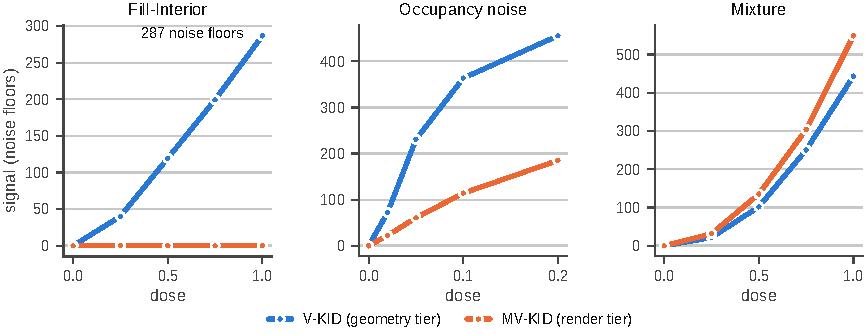
\includegraphics[width=0.95\linewidth]{figures/fig2_dose_response}
\caption{\textbf{Dose--response.} Each metric in units of its own noise floor,
which is the only scale on which the two are commensurable. Both rise
monotonically on occupancy noise and on the mixture axis; on the interior axis
the render metric does not move.}
\label{fig:dose}
\end{figure*}

% =====================================================================
\section{View Protocols}
\label{app:ablation}
% =====================================================================

\subsection{Encoders, view budgets and cutaways}

Table~\ref{tab:ablation} varies the encoder, the number and projection of the
views, and the cut, holding the statistic fixed.

\begin{table}[t]
\centering
\footnotesize
\caption{Separation of \solidify{} from real in each condition's own noise floors
($n{=}256$ against $512$ reference builds, paired subsample, $95\%$ intervals). \textbf{Every exterior condition lands
between $0.0$ and $0.2$ noise floors; cutaways reach $7$--$56$ with the same encoder and
the same statistic.}}
\label{tab:ablation}
\setlength{\tabcolsep}{3pt}
\resizebox{\linewidth}{!}{%
\begin{tabular}{llr@{\hspace{0.6em}}lc}
\toprule
& condition & \multicolumn{2}{c}{separation} & interior? \\
\midrule
\multirow{5}{*}{\rotatebox{90}{\footnotesize encoder}}
& DINOv2-B (ours) & $+0.2$ & {\footnotesize[0.1, 0.3]} & no \\
& CLIP ViT-B/16 & $+0.1$ & {\footnotesize[$-0.1$, 0.2]} & no \\
& CLIP ViT-B/32 & $+0.1$ & {\footnotesize[0.0, 0.2]} & no \\
& ResNet-50 (ImageNet-supervised) & $+0.0$ & {\footnotesize[$-0.1$, 0.1]} & no \\
& Inception-v3 pool3 (the FID backbone) & $+0.2$ & {\footnotesize[0.0, 0.3]} & no \\
\midrule
\multirow{3}{*}{\rotatebox{90}{\footnotesize views}}
& $8$ orthographic & $+0.2$ & {\footnotesize[0.1, 0.3]} & no \\
& $16$ orthographic & $+0.1$ & {\footnotesize[$-0.0$, 0.2]} & no \\
& perspective & $+0.1$ & {\footnotesize[$-0.0$, 0.2]} & no \\
\midrule
\multirow{4}{*}{\rotatebox{90}{\footnotesize \textbf{cut}}}
& \textbf{facing quadrant removed} & $\mathbf{+6.7}$ & {\footnotesize[5.9, 7.5]} & \textbf{yes} \\
& \textbf{vertical cross-sections} & $\mathbf{+14.0}$ & {\footnotesize[12.8, 15.2]} & \textbf{yes} \\
& \textbf{roof removed} & $\mathbf{+17.1}$ & {\footnotesize[15.3, 19.2]} & \textbf{yes} \\
& \textbf{floorplan cross-sections} & $\mathbf{+55.8}$ & {\footnotesize[52.4, 59.6]} & \textbf{yes} \\
\midrule
& \vkid{} (no rendering at all) & $+120.8$ & {\footnotesize[115.7, 126.3]} & yes \\
\bottomrule
\end{tabular}}
\end{table}

% Source: outputs/run_20261104_213620_view_facade_section (notes §76, results T90).
\subsection{Facade and cross-section views}
\label{app:views25d}

The corner views of \mvkid{} are one choice of exterior observation. We test two others,
holding the builds, the reference and the encoder of the $n{=}256$ leaderboard fixed
(every arm reproduces the leaderboard's build hashes). The \vkid{} column uses the
leaderboard's own noise floor. Each view condition draws its own floor from $48$ fresh real
draws, and for the corner views that draw comes out $1.22$ times the leaderboard's, so from
identical raw distances the corner column reads \matshuffle{} at $+346$ where the
leaderboard reads $+422.43$; on the leaderboard's floor the corner column reads \solidify{}
at $+0.35$, \hollow{} at $+0.04$ and \monochrome{} at $+535.36$. \emph{Facade
views} are the views an architect draws: four side elevations at zero elevation, alone
(A-sides) and with a roof plan (A-render), and the 2.5D facade representation itself,
five images of the first block along each axis shaded by its depth, drawn without a
renderer (A-2.5D). \emph{Cross-section views} open the build: one-voxel sections through
the middle of $x$, $z$ and $y$ seen face-on (B-mid), sections at $25$, $50$ and $75\%$ of
each axis (B-9), and the build with half removed along each axis, seen at the cut
(B-cut). Table~\ref{tab:views25d} reports every condition in its own noise floors above
the held-out real draw.

\begin{table}[h]
\centering
\small
\setlength{\tabcolsep}{3.5pt}
\resizebox{\linewidth}{!}{%
\begin{tabular}{lrrrrrrrr}
\toprule
 & corner & A-sides & A-render & A-2.5D & B-mid & B-9 & B-cut & \vkid{} \\
\midrule
\solidify{}   & $+0.3$   & $+4.4$   & $+3.6$   & $0$      & $+71.1$  & $+67.5$  & $+14.3$  & $+444.4$ \\
\hollow{}     & $+0.0$   & $+0.8$   & $+0.6$   & $0$      & $+39.7$  & $+42.8$  & $+5.3$   & $+265.4$ \\
\matshuffle{} & $+346$   & $+548$   & $+610$   & $+355$   & $+226$   & $+292$   & $+415$   & $0$ \\
\monochrome{} & $+439$   & $+1146$  & $+1309$  & $+314$   & $+1080$  & $+1314$  & $+925$   & $0$ \\
yaw $90^\circ$ & $-0.2$  & $+0.0$   & $+0.1$   & $+0.1$   & $+0.4$   & $+0.5$   & $-0.2$   & $0$ \\
mirror        & $-0.2$   & $+0.1$   & $+0.1$   & $+0.0$   & $-0.4$   & $-0.3$   & $+0.0$   & $0$ \\
\midrule
$\rho$ vs corner & $1$   & $0.97$   & $0.97$   & $0.96$   & $0.93$   & $0.93$   & $0.95$   & $0.27$ \\
$\rho$ vs \vkid{} & $0.27$ & $0.10$  & $0.10$   & $0.28$   & $0.07$   & $0.07$   & $0.05$   & $1$ \\
\bottomrule
\end{tabular}}
\caption{\textbf{Facade and cross-section views ($n{=}256$).} Separation in noise floors
above held-out real data. $\rho$: Spearman correlation of the ordering of eleven arms
(four probes, three procedural baselines, three autoregressive arms, Dream-Cubed) with
corner-view \mvkid{} and with \vkid{}. The A-2.5D images of \solidify{} and \hollow{} are
bit-identical to the real images for all $256$ builds.}
\label{tab:views25d}
\end{table}

\paragraph{Facade views do not see the interior.} The 2.5D facade images of \solidify{}
and \hollow{} are bit-identical to those of the real builds for all $256$ houses, so the
separation is exactly zero. The representation records the first block along each axis
and counts glass as a block, and a probe that keeps the exterior air region fixed keeps
every first block fixed. This is Lemma~\ref{lem:surface} with no
renderer involved. Rendered elevations read \solidify{} at $+4.4$ noise floors, above the
corner views' $+0.3$, because a face-on camera looks straight through windows into the
filled rooms; at $n{=}128$ the same condition reads $+2.3$. The signal is a window
leak, a hundred times smaller than the $444$ of \vkid{}, and \hollow{} stays below one
noise floor.

\paragraph{Cross-sections see the interior through appearance.} A one-voxel section shows
rooms as background and filled rooms as material, and B-mid separates \solidify{} by
$+71$ and \hollow{} by $+40$ noise floors. Removing half of the build (B-cut) leaves the
far walls in view and reaches $+14$. Both are far below \vkid{}, and the ordering of the
other arms barely moves: every view condition ranks the eleven arms as the corner views
do ($\rho \ge 0.93$) and unlike \vkid{} ($\rho \le 0.28$), with \monochrome{} and the
procedural baselines furthest from real. Showing the inside to an image encoder recovers
the interior signal without turning the metric into a structural one, which is the
complementary blindness that motivates scoring each pillar separately
(\mainsec{sec:complementary}).

\paragraph{Invariance.} Axis-aligned views are not invariant to the heading of a build
unless the pooled set is. Under a $90^\circ$ yaw and a mirror of the held-out real builds,
every condition moves by at most $0.5$ noise floors, so mean-pooling over the sides is
invariant in practice.


% =====================================================================
\section{What a Render Protocol Provably Cannot See}
\label{app:hull}
% =====================================================================

%TL;DR of paragraph: a deterministic renderer induces equivalence classes on which every render-and-embed metric is constant.
A deterministic render pipeline $R_V$ with a fixed view set $V$ induces an
equivalence relation on structures: $x \sim x'$ exactly when
$R_V(x) = R_V(x')$.

\begin{lemma}[Render kernel]\label{lem:kernel}
If $x \sim x'$ then $T(\mathcal{E}(R_V(x))) = T(\mathcal{E}(R_V(x')))$ for every
encoder $\mathcal{E}$, every pooling rule and every statistic $T$.
\end{lemma}
\begin{proof}
Immediate: the composition is a function of $R_V(x)$ alone.
\end{proof}

%TL;DR of paragraph: the lemma is only interesting because our own probe lands inside a class, which needs two more facts.
On its own Lemma~\ref{lem:kernel} is a tautology. It becomes a statement about
this paper because \solidify{} lands inside an equivalence class, which needs
two further facts.

\begin{lemma}[Surface invariance]\label{lem:surface}
\solidify{} leaves the exterior-air region unchanged, and leaves every exterior
face unchanged in cell, direction and material.
\end{lemma}

\begin{lemma}[Occlusion]\label{lem:occl}
Assume (a) nearest-surface shading, (b) faces bordering exterior air are opaque,
and (c) every camera lies outside the bounding box. Then
$R_V(\solidify(x)) = R_V(x)$ for \emph{every} view set $V$.
\end{lemma}
\begin{proof}[Proof sketch]
Any ray reaching a newly filled cell must first cross a face bordering exterior
air. By (b) that face is opaque and by (a) it is what the ray returns, so no
pixel can depend on the filled interior.
\end{proof}

%TL;DR of paragraph: the surface-invariance lemma also kills point-cloud and chamfer metrics, exactly.
Lemma~\ref{lem:surface} has a consequence beyond rendering. Any metric computed
on samples of the \emph{exterior surface} is a function of that face set, so it
too is constant under \solidify{}. We verify it: sampling exterior face centers
from a build and from its solidified copy gives \textbf{identical point sets on
$128$ of $128$ builds}, so chamfer distance, earth-mover distance and every
other point-cloud distance between them is exactly zero. This matters for the
proposal to replace renders with surface samples
\citep{luan2026rendermetric}, and for this corpus in particular: the model
released with it \citep{chen2019voxelcnn} reports a cumulative chamfer distance.
Sampling \emph{all} exposed faces, including those bordering sealed cavities,
does see the probe (mean chamfer $0.485$), but a surface sampler that reached
interior cavity walls would be observing the interior, which is the thing at
issue.

%TL;DR of paragraph: the conclusion, and the measurement that separates the exact regime from the leaky one.
Together with Lemma~\ref{lem:kernel} this is an impossibility result, not a
statistical one: under an opaque renderer \emph{no} encoder, statistic, sample
size or view budget separates a corpus from its solidified copy. We verify
Lemma~\ref{lem:surface} exhaustively ($0$ violations over the $399$ held-out
builds, and $0$ for \hollow{}) and Lemma~\ref{lem:occl} by rendering all $1{,}596$
test-split views through counterfactual pipelines that switch each leak off in turn.
\emph{Fixed atlas} packs one texture atlas for the whole experiment, so no texture
coordinate depends on which faces a build has:

\begin{center}\small
\resizebox{\linewidth}{!}{%
\begin{tabular}{lrrrr}
\toprule
renderer & bit-identical & px changed (med.) & max ch.\ (med.) & \mvkid{}, $n{=}256$ \\
\midrule
glass opaque, fixed atlas, CPU raster (Lemma~\ref{lem:occl}) & $\mathbf{100.0\%}$ & --- & --- & $\mathbf{0}$ \\
glass opaque, fixed atlas, GPU raster & $88.9\%$ & $0.008\%$ & $1$ & $-0.00004$ \\
glass opaque, per-build atlas & $8.1\%$ & $0.99\%$ & $79$ & --- \\
translucent, fixed atlas & $41.3\%$ & $0.21\%$ & $107$ & $+0.40$ \\
\textbf{deployed} (translucent, per-build atlas) & $9.1\%$ & $1.23\%$ & $128$ & $+0.29$ \\
\bottomrule
\end{tabular}}
\end{center}

%TL;DR of paragraph: our renderer violates hypothesis (b) twice, once physically and once as an artifact we disclose.
Our renderer violates hypothesis (b) in two ways, and the two have different
standing. The first is physical: Minecraft glass is translucent, so a
window in front of a filled void reveals the fill. This is a real channel, and
it alone alters $59\%$ of views. The second is an artifact of our mesh builder,
which we report because it inflates that count. \texttt{build\_mesh} assigns
texture-atlas tiles in face-iteration order over \emph{all} exposed faces,
interior ones included; deleting interior faces can change the tile order, hence
the atlas layout, hence every UV rectangle, and the sampler is nearest-neighbor.
With glass opaque this alone alters $92\%$ of views. A reader should
therefore take $91\%$ as a property of our renderer, not of the corruption; the
corruption's own reach is the $59\%$ that survives fixing the atlas. Counted per
house, the fill shows in at least one view of $67\%$ of houses with the atlas
fixed and of $92\%$ under the deployed renderer. The GPU
rasterizer adds a third, numerical channel: it is not bit-reproducible, and
rendering the same build twice changes up to $9$ pixels by $1/255$ in $6$ of $24$
houses. Across the test split this reaches at most $2/255$ on $0.01\%$ of pixels
and moves \mvkid{} by $4\times10^{-5}$ noise floors; the CPU rasterizer has none.
On LEGO, whose wool is opaque, the deployed renderer's $-0.01$ for \solidify{}
becomes $-0.00004$ with the atlas fixed.

%TL;DR of paragraph: rescoring the probe through all four renderers shows the residual is wobble, not partial detection.
We then rescored the probe end to end through each of the four pipelines, holding
the arms, the draw and the estimator fixed and changing only the texture pack.
This turns the lemma into a prediction the benchmark either satisfies or does
not:

\begin{center}\small
\begin{tabular}{lrc}
\toprule
renderer & \mvkid{} separation & features identical \\
\midrule
opaque, flat tiles & $\mathbf{+0.000}$ & \textbf{yes} \\
flat tiles, translucency on & $-0.069$ & no \\
textured, translucency off & $+0.026$ & no \\
deployed & $+0.119$ & no \\
\bottomrule
\end{tabular}
\end{center}

The prediction holds exactly: bit-identical renders give bit-identical features
and therefore an identical kernel distance, so the separation is $0$ as an
identity rather than as a rounded measurement. The other three rows carry the
more useful lesson. The residual the benchmark reports for this probe is not a
small signal. It is \emph{wobble}. Changing only the texture pack, which
changes nothing whatever about the geometry being probed, moves it from $+0.119$
to $+0.026$ to $-0.069$: a range wider than the value itself, and one that crosses
zero, with the probe reading \emph{closer} to real than real does. This is what
it looks like when a metric is flat on an axis rather than weakly sensitive to
it, and it is why we argue the point by magnitude and ordering rather than by
the residual's sign. (The deployed row reads $+0.119$ here against the
protocol run's $+0.14$ for the same raw values, $-0.0018$ and $-0.0014$; the two runs
estimate their own floors, $0.00337$ and $0.00289$, which is the effect
Sec.~\ref{app:nscale} documents.)

%TL;DR of paragraph: where the surviving signal is lost, stated as measurement rather than theory.
Where a leaked signal is lost is a measurement rather than a theorem. In DINOv2
the patch tokens a changed pixel touches move by $12\%$ of the between-build
scale, the CLS token by $3.9\%$ and the four-view pooled embedding by $2.0\%$, so
the signal enters the features and is attenuated by aggregation rather than
ignored by the encoder.

%TL;DR of paragraph: the converse lemma, which makes the complementary-blindness claim symmetric.
The converse holds by the same style of argument and makes the paper's
complementarity claim provable on both sides rather than measured on one.

\begin{lemma}[Material blindness of \vkid{}]\label{lem:matblind}
The descriptor of Sec.~\ref{sec:metrics} factors through the occupancy mask, so any
transformation preserving occupancy, \matshuffle{} and \monochrome{} among them,
leaves
it pointwise unchanged, and \vkid{} returns the real arm's value exactly.
\end{lemma}

Verified: descriptors are bit-identical (max difference $0.0$) and \vkid{}
returns the identical float for all three arms. The $+0.00$ printed in
\maintab{tab:leaderboard} is an identity, not a rounded measurement. Renders
of those same builds are never identical ($0$ of $256$ views; a median $25\%$ of
pixels move), so material permutation provably escapes the render kernel exactly
as interior fill provably falls inside it.

% =====================================================================
\section{Other Observers: Point Clouds, Structural Metrics, a VLM Judge}
\label{app:probe3d}
% =====================================================================

\subsection{3D-native metrics and their samplers}

We score two learned point-cloud encoders, Uni3D-B and ULIP-2 PointBERT ($10$k points with
color, each repository's preprocessing), and two point-set distances, chamfer on $2{,}048$
points and exact EMD on $512$, each under three samplers. \emph{all} samples uniformly by
area over every face, the default of Uni3D, ULIP-2, PointFlow-style MMD and FPD.
\emph{vis} samples only faces an exterior orthographic ray hits first, which is what a
watertight-mesh or rendered-depth pipeline observes. \emph{cut} samples the faces the four
cutaway views show. Minecraft builds become meshes with one quad per block face bordering
air. The Objaverse set is $290$ buildings passing a strict multi-room rule (hidden area
$\geq 30\%$, hidden volume $\geq 5\%$, at least two sealed spaces), scored at $n{=}96$
against $130$ reference objects; \emph{strip} removes every hidden face and \emph{fill}
replaces the hidden volume by a solid, with an exterior pixel change of $0.04/255$. The
Minecraft ladder is scored at $n{=}128$ against $248$ reference builds. Cells are
null-standardized $z$-scores, seed 0\,/\,seed 1; seed changes the split, the probe draw and
every sampler draw.

\begin{table*}[t]
\centering
\footnotesize
\caption{\textbf{Every 3D-native metric inherits the null space of its sampler.}
Separation from held-out real (noise floors, seed 0\,/\,seed 1). Under \emph{vis} every
point-cloud row is blind to both interior probes on both domains, within $1.6$ floors in
every cell; under \emph{all} and \emph{cut} the learned encoders see them.}
\label{tab:probe3d}
\begin{tabular}{lrrrrr}
\toprule
\multicolumn{6}{l}{\textbf{Objaverse multi-room buildings}, $n{=}96$} \\
metric & strip & fill & noise & missing wall & decimate \\
\midrule
DINOv2, 4 ext.\ views, KID & $+0.0$\,/\,$+0.0$ & $+0.0$\,/\,$+0.0$ & $+34.7$\,/\,$+66.6$ & $+9.5$\,/\,$+15.0$ & $+21.3$\,/\,$+29.0$ \\
DINOv2, 4 cutaways, KID & $+10.9$\,/\,$+9.0$ & $+13.5$\,/\,$+13.7$ & $+43.9$\,/\,$+32.7$ & $+7.0$\,/\,$+6.2$ & $+22.3$\,/\,$+14.6$ \\
\vkid{} & $+23.7$\,/\,$+26.5$ & $+73.8$\,/\,$+118.4$ & $+18.1$\,/\,$+31.8$ & $+16.2$\,/\,$+13.4$ & $+12.0$\,/\,$+12.4$ \\
Uni3D KID, \emph{all} & $+4.6$\,/\,$+11.5$ & $+8.5$\,/\,$+14.1$ & $+13.7$\,/\,$+34.0$ & $+9.8$\,/\,$+15.4$ & $+4.3$\,/\,$+6.7$ \\
Uni3D KID, \emph{vis} & $+0.4$\,/\,$-0.2$ & $+0.3$\,/\,$+0.0$ & $+9.5$\,/\,$+20.7$ & $+16.5$\,/\,$+18.5$ & $+7.9$\,/\,$+8.3$ \\
Uni3D KID, \emph{cut} & $+4.3$\,/\,$+8.4$ & $+6.3$\,/\,$+12.4$ & $+3.7$\,/\,$+13.2$ & $+5.6$\,/\,$+10.0$ & $+1.9$\,/\,$+2.9$ \\
ULIP-2 KID, \emph{all} & $+2.4$\,/\,$+4.2$ & $+3.3$\,/\,$+8.4$ & $+5.0$\,/\,$+19.6$ & $+12.5$\,/\,$+29.7$ & $+7.8$\,/\,$+14.0$ \\
ULIP-2 KID, \emph{vis} & $-0.0$\,/\,$-0.3$ & $+0.1$\,/\,$-0.1$ & $+6.5$\,/\,$+16.3$ & $+15.2$\,/\,$+22.4$ & $+9.3$\,/\,$+10.9$ \\
ULIP-2 KID, \emph{cut} & $+4.2$\,/\,$+4.7$ & $+4.9$\,/\,$+10.8$ & $+3.5$\,/\,$+11.5$ & $+8.4$\,/\,$+18.8$ & $+5.1$\,/\,$+6.0$ \\
chamfer MMD, \emph{all} & $+3.4$\,/\,$+3.9$ & $-0.6$\,/\,$-0.4$ & $-0.3$\,/\,$+0.0$ & $+9.9$\,/\,$+10.9$ & $+0.2$\,/\,$+1.4$ \\
chamfer MMD, \emph{vis} & $-0.1$\,/\,$+0.2$ & $-0.0$\,/\,$+0.1$ & $-0.6$\,/\,$-0.6$ & $+7.9$\,/\,$+10.5$ & $-0.9$\,/\,$+0.3$ \\
chamfer MMD, \emph{cut} & $+2.8$\,/\,$+2.9$ & $-0.7$\,/\,$-0.1$ & $-0.2$\,/\,$+0.1$ & $+8.8$\,/\,$+7.7$ & $+0.2$\,/\,$+0.9$ \\
EMD MMD, \emph{all} & $+3.4$\,/\,$+3.8$ & $+0.7$\,/\,$+0.2$ & $+3.7$\,/\,$+2.3$ & $+19.6$\,/\,$+20.5$ & $+0.9$\,/\,$+1.7$ \\
EMD MMD, \emph{vis} & $-0.0$\,/\,$+0.2$ & $-0.2$\,/\,$+0.3$ & $+0.5$\,/\,$+0.9$ & $+11.6$\,/\,$+9.9$ & $+0.4$\,/\,$+0.6$ \\
EMD MMD, \emph{cut} & $+2.2$\,/\,$+3.3$ & $-0.1$\,/\,$-0.1$ & $+0.6$\,/\,$+0.8$ & $+13.2$\,/\,$+15.2$ & $+0.5$\,/\,$+1.0$ \\
\midrule
\multicolumn{6}{l}{\textbf{Minecraft houses}, $n{=}128$} \\
metric & \solidify{} & \hollow{} & canon-16 & $40\%$ deleted & \matshuffle{} \\
\midrule
Uni3D KID, \emph{all} & $+21.7$\,/\,$+22.6$ & $+8.5$\,/\,$+9.6$ & $+154.8$\,/\,$+186.0$ & $+50.9$\,/\,$+65.4$ & $+16.5$\,/\,$+18.9$ \\
Uni3D KID, \emph{vis} & $-0.1$\,/\,$+0.4$ & $+0.1$\,/\,$+0.4$ & $+128.2$\,/\,$+117.1$ & $+46.0$\,/\,$+43.1$ & $+19.0$\,/\,$+16.0$ \\
Uni3D KID, \emph{cut} & $+37.0$\,/\,$+30.4$ & $+13.5$\,/\,$+10.4$ & $+132.3$\,/\,$+117.9$ & $+43.6$\,/\,$+49.8$ & $+19.1$\,/\,$+15.8$ \\
ULIP-2 KID, \emph{all} & $+4.0$\,/\,$+3.2$ & $+2.1$\,/\,$+1.9$ & $+70.2$\,/\,$+63.0$ & $+49.1$\,/\,$+48.1$ & $+33.6$\,/\,$+27.0$ \\
ULIP-2 KID, \emph{vis} & $-0.1$\,/\,$+0.1$ & $-0.1$\,/\,$+0.0$ & $+62.1$\,/\,$+60.8$ & $+41.0$\,/\,$+45.0$ & $+30.6$\,/\,$+26.6$ \\
ULIP-2 KID, \emph{cut} & $+9.8$\,/\,$+6.4$ & $+2.2$\,/\,$+1.3$ & $+52.5$\,/\,$+41.8$ & $+34.3$\,/\,$+30.8$ & $+22.9$\,/\,$+15.0$ \\
chamfer MMD, \emph{all} & $+6.3$\,/\,$+8.0$ & $+1.1$\,/\,$+1.7$ & $+55.0$\,/\,$+66.2$ & $+13.1$\,/\,$+15.9$ & $-0.0$\,/\,$+0.2$ \\
chamfer MMD, \emph{vis} & $-0.1$\,/\,$-0.1$ & $-0.4$\,/\,$-0.3$ & $+64.3$\,/\,$+75.2$ & $+8.0$\,/\,$+9.5$ & $-0.2$\,/\,$-0.1$ \\
chamfer MMD, \emph{cut} & $+7.8$\,/\,$+6.9$ & $+1.8$\,/\,$+1.4$ & $+55.6$\,/\,$+51.2$ & $+14.9$\,/\,$+14.0$ & $+0.0$\,/\,$-0.2$ \\
EMD MMD, \emph{all} & $+4.5$\,/\,$+3.6$ & $+1.0$\,/\,$-0.0$ & $+36.5$\,/\,$+31.8$ & $+11.2$\,/\,$+8.8$ & $-0.3$\,/\,$-0.7$ \\
EMD MMD, \emph{vis} & $+0.0$\,/\,$+0.6$ & $+0.0$\,/\,$+0.1$ & $+40.7$\,/\,$+45.9$ & $+10.5$\,/\,$+11.1$ & $-0.0$\,/\,$+0.1$ \\
EMD MMD, \emph{cut} & $+3.6$\,/\,$+3.9$ & $+0.4$\,/\,$+0.4$ & $+27.0$\,/\,$+31.6$ & $+8.9$\,/\,$+9.5$ & $+0.1$\,/\,$-0.7$ \\
\bottomrule
\end{tabular}
\end{table*}

The reading is the same on both domains. Under \emph{vis} the learned encoders still
separate exterior damage at $5$ to $188$ floors, so they are not insensitive; they are given
no interior to see. Under \emph{all} and \emph{cut}, Uni3D sees filled Minecraft interiors
at $22$ to $37$ floors and ULIP-2 more weakly. Chamfer and EMD stay at or below about $8$
floors even when their points include the interior. Generated meshes from surface-fitted or
score-distillation generators are exterior shells, so on them \emph{all} and \emph{vis}
coincide and a learned 3D metric is blind in practice as well. Seed agreement is Pearson
$0.91$ over $275$ Objaverse cells and $0.98$ over $336$ Minecraft cells.

% Source: outputs/run_20261104_235615_bench_headtohead (notes §80, results T92).
\subsection{\vkid{} against structural alternatives}
\label{app:headtohead}

Render metrics are blind to interiors by construction, so outscoring them is not what a
geometry pillar must show. We therefore compare \vkid{} against the structural metrics a
3D reviewer would reach for, under the tests \vkid{} itself passed. The rows are:
\begin{itemize}
\item kernel distances on the 3D encoders Uni3D and ULIP-2, fed points from every exposed
  block face, sealed rooms included (\emph{all}), or uniform points inside occupied voxels
  (\emph{vol});
\item the set statistics of the shape-generation literature, MMD, $1-$coverage and
  1-NN accuracy, under chamfer and exact EMD on all-face points, chamfer on voxel centres,
  and $1-$IoU between occupancy grids, either aligned at the bounding-box corner or
  maximised over the eight yaw and mirror variants;
\item KID on the occupancy grid itself, bounding-box centred in $32^3$ and $4^3$
  average-pooled. This is the same estimator as \vkid{}, with raw occupancy as the
  features.
\end{itemize}

Each row is scored by the ladder code that gates the leaderboard. That ladder uses the
houses\_32 ladder subset, $n{=}128$, 48 noise draws and the geometry rungs. The encoders,
which read colour, are also judged on the render rungs. Each row is then scored on the
$n{=}256$ arms of the leaderboard of record, rebuilt with matching build hashes. The
\vkid{} row reproduces the leaderboard exactly ($+444.4$).

\begin{table}[h]
\centering
\small
\setlength{\tabcolsep}{2.5pt}
\resizebox{\linewidth}{!}{%
\begin{tabular}{lrrrrlrrr}
\toprule
 & \multicolumn{4}{c}{ladder, $n{=}128$} & & \multicolumn{3}{c}{board, $n{=}256$} \\
\cmidrule(lr){2-5}\cmidrule(lr){7-9}
row & \solidify{} & \hollow{} & \matshuffle{} & \monochrome{} & gates & \solidify{} & $\rho$ \vkid{} & $\rho$ \mvkid{} \\
\midrule
\textbf{\vkid{}}            & $\mathbf{+111.4}$ & $\mathbf{+71.0}$ & $0$ & $0$ & \textbf{pass} & $\mathbf{+444.4}$ & $1$ & $0.27$ \\
occupancy KID               & $+48.4$  & $+13.1$ & $0$     & $0$      & G2, G6 & $+121.2$ & $0.83$ & $0.23$ \\
Uni3D KID, all              & $+26.6$  & $+10.4$ & $+22.4$ & $+99.7$  & G6     & $+31.8$  & $0.51$ & $0.85$ \\
Uni3D KID, vol              & $+37.2$  & $+10.6$ & $+6.7$  & $+105.5$ & G6     & $+108.4$ & $0.59$ & $0.78$ \\
ULIP-2 KID, all             & $+4.6$   & $+1.8$  & $+29.1$ & $+101.8$ & G6 / G2 & $+12.0$ & $0.42$ & $0.87$ \\
ULIP-2 KID, vol             & $+11.9$  & $+9.0$  & $+9.7$  & $+62.8$  & G6 / G2 & $+43.2$ & $0.51$ & $0.85$ \\
chamfer MMD, all            & $+7.6$   & $+1.4$  & $-0.1$  & $-0.1$   & G2, G8 & $+8.9$   & $0.64$ & $0.27$ \\
chamfer 1-NNA, all          & $+2.9$   & $+1.1$  & $0.0$   & $-0.6$   & G2, G6 & $+4.0$   & $0.76$ & $0.43$ \\
EMD MMD, all                & $+3.2$   & $+0.3$  & $-0.2$  & $-0.3$   & G2, G8 & ---      & ---    & ---    \\
EMD 1-NNA, all              & $+1.6$   & $+0.1$  & $-0.5$  & $-0.2$   & G2     & ---      & ---    & ---    \\
chamfer MMD, voxel centres  & $-3.4$   & $+2.8$  & $+0.1$  & $+0.1$   & G2, G8 & $-3.5$   & $0.53$ & $0.54$ \\
IoU MMD, D4-aligned         & $-9.0$   & $+7.7$  & $0$     & $0$      & G8     & $-5.3$   & $0.36$ & $0.35$ \\
IoU 1-NNA, D4-aligned       & $+2.7$   & $+2.4$  & $0$     & $0$      & G2     & $+5.9$   & $0.75$ & $0.28$ \\
IoU MMD, corner             & $-11.5$  & $+8.4$  & $0$     & $0$      & G6, G8 & $-7.4$   & $0.52$ & $0.46$ \\
\bottomrule
\end{tabular}}
\caption{\textbf{\vkid{} against structural alternatives.} Separation from held-out real
data in each row's own noise floors. Gates: G2 noise ordering, G6 invariance, G8
$n$-stability; ``G6 / G2'' gives the failing gate under the geometry and the render rungs.
$\rho$: Spearman correlation of the ordering of eleven leaderboard arms. The $1-$coverage
rows fail at least two gates each and are omitted. Exact EMD runs on the ladder only. The
ladder scores against its $248$-build subset reference and measures from the null mean, so \vkid{} reads $+111.4$ there
and $+201.8$ in the protocol run at the same $n$.}
\label{tab:headtohead}
\end{table}

\paragraph{Of these rows, only \vkid{} passes every gate.} It separates \solidify{} $2.3\times$ more
strongly than the next row and \hollow{} $5\times$ more strongly, and appearance and
rotation leave it unmoved. The nearest alternative is occupancy KID: the same estimator on
the raw grid. It sees \solidify{} and orders the leaderboard much as \vkid{} does
($\rho{=}0.83$), but it fails noise ordering. Its rotation reading also sits at the edge of
the invariance bar, because a centred grid is not yaw-invariant. What \vkid{} adds is the
D4-invariant local descriptor, not the estimator, and generic orbit-averaged occupancy
descriptors pass as well (Sec.~\ref{app:vkid-robust}), so the class that passes is the
D4-invariant occupancy kernel distance, of which \vkid{} is one instance.

\paragraph{3D encoders see the interior once their points include it, but read
appearance.} On interior-inclusive points Uni3D and ULIP-2 separate both probes, so their
blindness in Table~\ref{tab:probe3d} belongs to the visible-surface sampler and not to the
encoders. They are not geometry metrics, however. \matshuffle{} and \monochrome{}, which
leave occupancy unchanged, move them by up to $106$ noise floors at $n{=}128$. Uni3D is
not yaw-invariant (a $90^\circ$ turn moves it on volume points by $+5.7$ floors at
$n{=}256$), and both rank the
leaderboard as \mvkid{} does ($\rho \ge 0.78$). As a geometry pillar they would let a
generator trade structure for appearance, which the worst-pillar aggregation exists to
prevent.

\paragraph{The voxel-generation suite misses the probes or rewards the fill.} Chamfer,
EMD and IoU set statistics never separate the interior probes by more than single digits,
and each fails noise ordering or $n$-stability. Nearest-neighbour MMD under IoU or
voxel-centre chamfer goes further and places \solidify{} \emph{closer} to the reference
than held-out real data, by $3$ to $12$ noise floors. A filled house overlaps its
neighbours more than a house with rooms does. The metric the voxel literature reports
would therefore reward a generator for filling its interiors.

\paragraph{Cost.} On about $3{,}000$ to $4{,}400$ builds, \vkid{} takes $15$ to $18$\,s on
one CPU process. Each encoder takes $25$ to $50$\,s of GPU time after sampling, chamfer
takes $2$ to $3$ minutes of GPU time, and exact EMD on $512$ points took $32$ minutes on
$16$ CPU cores.


\subsection{The VLM judge}
\label{app:vlm}

The judge is \texttt{gpt-4o-2024-11-20} at temperature $0$, shown two builds as four
exterior (or cutaway) views each and asked which is the more realistic house, with both
presentation orders and a plan registered before any call. Only 3D-Craft builds and probes
derived from them reach the API. $2{,}288$ trials, all valid. Each build is one image, its
four views at azimuths $45^\circ$, $135^\circ$, $225^\circ$ and $315^\circ$ in a $2{\times}2$
grid. The system prompt is \enquote{You are an experienced Minecraft player judging builds
for a research benchmark. You always answer with a single JSON object.} The user message
is the question, then \enquote{Build A:} and its image, then \enquote{Build B:} and its
image, where the question reads \enquote{Two Minecraft builds, A and B, are shown below.
\textless view note\textgreater{} Which looks more like a real Minecraft house, as built by
a player? You must pick one; ``equal'' is not allowed. Reply with only a JSON object:
\texttt{\{"choice": "A" or "B", "reason": "<at most 20 words>"\}}}. The view
note is \enquote{Each image shows one build from four viewing angles (a 2x2 grid of
exterior views).} for exterior pairs, and for cutaways states that the upper half of the
build, or in each view the corner facing the camera, has been removed so the reader can
see inside. The registered predictions were chance for both interior probes on exterior
views, above chance for both on cutaways, certainty against \randomvox{}, and a
preference for \gabled{} over \patchstitch{}.

\begin{table}[h]
\centering
\small
\setlength{\tabcolsep}{3pt}
\caption{Probability the judge prefers the first arm, with cluster-bootstrap $95\%$
intervals. Every pre-registered prediction holds except the last, where the judge agrees
with both metrics.}
\label{tab:vlm}
\resizebox{\linewidth}{!}{%
\begin{tabular}{llrl}
\toprule
pair & view & $n$ & P(first) \\
\midrule
real vs \solidify{} & exterior & $256$ & $0.53$ $[0.50, 0.56]$ \\
real vs \solidify{} & roof off & $256$ & $0.70$ $[0.64, 0.75]$ \\
real vs \solidify{} & quadrant cut & $128$ & $0.63$ $[0.53, 0.72]$ \\
real vs \hollow{} & exterior & $256$ & $0.52$ $[0.49, 0.54]$ \\
real vs \hollow{} & roof off & $128$ & $0.73$ $[0.66, 0.80]$ \\
real vs \randomvox{} & exterior & $128$ & $1.00$ $[1.00, 1.00]$ \\
\gabled{} vs \patchstitch{} & exterior & $256$ & $0.28$ $[0.21, 0.35]$ \\
\bottomrule
\end{tabular}}
\end{table}

On exterior views of a house and its filled twin the judge picks the first slot $93\%$ of
the time and the two orders agree on only $13\%$ of pairs, so its preference there is
position, not content. Houses whose fill shows through a window do not move it ($0.53$
against $0.50$ for the rest). At the system level a
Bradley--Terry fit over eleven arms ranks held-out real sixth, with \solidify{} and both
\voxar{} arms above it. Its Spearman agreement with the $n{=}256$ leaderboard is $0.74$ for
\mvkid{}, $0.54$ for \blockscore{} and $0.20$ for \vkid{} ($0.76$, $0.57$ and $0.16$ at
$n{=}128$), over 3D-Craft subsets for the judge and full scored sets for the metrics. The
judge reads exterior views and shares the render metric's null space, so we report it as a
third exterior observer rather than as ground truth.

% =====================================================================
\section{Robustness of \vkid{}}
\label{app:vkid-robust}
% =====================================================================

A hand-designed descriptor invites the objection that its features were chosen to catch
our probes. We answer it at two sample sizes: by deleting the two suspect terms at the
protocol run's $n{=}128$, and by removing whole families, drawing random subsets and
replacing the descriptor with generic maps at the leaderboard's $n{=}256$.

\subsection{The two suspect terms}
\label{app:descriptor}

The two objections are that \vkid{} separates \solidify{} only because the probe
adds mass and the descriptor carries an explicit size term, or only because the
descriptor carries a sealed-interior scalar the probe drives to zero.
Table~\ref{tab:descriptor-ablation} deletes both terms, alone and together, and
each block of the descriptor in turn, with $48$ fresh real draws per variant,
each separation in that variant's own noise floor. Neither term carries the
result, and the mass-matched \growshell{} column separates as strongly as
\solidify{}.

\begin{table}[t]
\centering
\small
\caption{Descriptor ablation, $n{=}128$, $48$ real draws per variant. Each
separation is in that variant's own noise floor, measured under that variant.
The two suspect terms are the explicit size scalar and the sealed-interior
scalar; deleting either or both leaves the separation intact.}
\label{tab:descriptor-ablation}
\setlength{\tabcolsep}{3pt}
\resizebox{\linewidth}{!}{%
\begin{tabular}{lrrrr}
\toprule
descriptor variant & dims & floor & \solidify{} & \growshell{} \\
\midrule
full                              & $77$ & $0.1097$ & $\mathbf{201.8}$ & $214.5$ \\
\midrule
\multicolumn{5}{l}{\emph{deleting a suspect term}} \\
without \texttt{log1p\_n\_blocks}       & $76$ & $0.1114$ & $202.2$ & $214.9$ \\
without \texttt{interior\_ratio\_sealed}& $76$ & $0.1127$ & $197.1$ & $211.7$ \\
without both                            & $75$ & $0.1147$ & $197.3$ & $211.9$ \\
\midrule
\multicolumn{5}{l}{\emph{deleting a whole block}} \\
without pattern bins    & $22$ & $0.5113$ & $198.0$ & $120.9$ \\
without wall thickness  & $72$ & $0.1163$ & $176.4$ & $216.6$ \\
without height profile  & $69$ & $0.1312$ & $199.6$ & $213.9$ \\
without global scalars  & $68$ & $0.1302$ & $171.6$ & $206.7$ \\
\midrule
\multicolumn{5}{l}{\emph{one block alone}} \\
pattern bins only       & $55$ & $0.1802$ & $113.9$ & $201.3$ \\
wall thickness only     & $5$  & $6.0167$ & $158.7$ & $75.7$ \\
height profile only     & $8$  & $1.6293$ & $8.0$   & $28.9$ \\
global scalars only     & $9$  & $1.7594$ & $164.5$ & $118.1$ \\
\bottomrule
\end{tabular}}
\end{table}

% Source: outputs/run_20261106_193358_vkid_robustness (notes §82, results T105).
\subsection{Families, random subsets and generic descriptors}

Each test below runs under the bench's own scoring code: the blocking gates on the ladder
($n{=}128$, $48$ fresh real draws, geometry rungs) and the separations on the $n{=}256$
leaderboard of record, whose build hashes we verify. Every row is whitened on the reference
and scored by the same unbiased KID, and every separation is in that row's own noise floor.
Rank agreement is Spearman's $\rho$ over the nine structural arms of the board against full
\vkid{}.

\paragraph{No family carries the result.}
We group the $77$ dimensions into seven families: $55$ pattern orbits, thickness ($5$
bins and $2$ scalars), height ($8$ bins and the entropy), surface ($2$), symmetry ($1$),
interior ($2$) and size ($1$). Removing any one family keeps every gate passing,
\solidify{} between $310$ and $457$ floors (full $444.4$), \hollow{} between $146$ and
$270$ (full $265.4$), and $\rho \geq 0.95$ (Table~\ref{tab:vkid-robust}). Random subsets
tell the same story without any grouping of ours: $20$ of $20$ random $38$-dimensional
subsets pass every gate, with \solidify{} at a median of $351$ floors (minimum $283$),
\hollow{} at $221$ ($133$) and $\rho$ at $0.97$ ($0.88$). At $19$ dimensions, $17$ of $20$
pass, and the weakest still separates \solidify{} by $179$ floors.

\paragraph{A descriptor with no hand design passes.}
We replace the descriptor by generic maps $\phi$ of the occupancy grid, made exactly
invariant to the yaw group by orbit averaging, $f(x) = \tfrac{1}{8}\sum_{g \in D_4}
\phi(gx)$, which is the only design step they share. Three are random-weight
three-layer 3D CNNs with mean and max pooling per layer ($224$ dimensions, three weight
draws), one is a feature-hashed histogram of raw $3^3$ occupancy patterns ($256$), and one
counts occupied $3^3$ neighbours of solid and air cells at $1\times$, $2\times$ and
$4\times$ pooling ($168$). All six rows, including the concatenation of a CNN with the
counts, pass every gate and separate \solidify{} by $257$ to $437$ floors and \hollow{} by
$166$ to $297$. Occupancy KID on a centred, pooled grid fails noise ordering and
invariance (Sec.~\ref{app:headtohead}); orbit averaging is what turns the raw volume into
a valid metric, and the separation follows from observing the volume rather than from
the choice of features. The generic rows reproduce \vkid{}'s ordering of probes and
baselines ($\rho$ between $0.8$ and $1.0$ over five arms) and differ from it in the
order of the four learned arms, where the random CNNs place Dream-Cubed behind the three
autoregressive arms; we report \vkid{} as the instantiation, and the ordering of close
learned arms as descriptor-dependent.

\paragraph{Global coherence is a separate axis.}
\patchstitch{} tiles $8^3$ patches of different real builds, so it is the natural attack
on a local descriptor. \vkid{} places it $368.2$ floors from real, fourth of nine arms.
Appending global terms, the largest 26-connected part ratio and component count, or
$2^3$ orbit histograms of the $2\times$ and $4\times$ max-pooled grid, keeps every gate
and leaves it fourth, with its separation between $0.73$ and $0.81$ of \solidify{}'s
($0.83$ for \vkid{}). The connected-part ratio on its own separates \patchstitch{} by
$258$ floors and both interior probes by none, so coherence is measurable and orthogonal
to the interior axis; at two of $79$ dimensions it does not move the joint kernel. We
keep \vkid{} unchanged and state its scope as local geometry.

\begin{table}[t]
\centering
\small
\caption{\vkid{} robustness. Gates on the ladder ($n{=}128$); separations on the
$n{=}256$ board in each row's own noise floor; $\rho$: Spearman over nine arms against
full \vkid{}. Random rows give the median and, in brackets, the minimum over $20$ draws.}
\label{tab:vkid-robust}
\setlength{\tabcolsep}{3pt}
\resizebox{\linewidth}{!}{%
\begin{tabular}{lrcrrrr}
\toprule
descriptor & dims & gates & \solidify{} & \hollow{} & \patchstitch{} & $\rho$ \\
\midrule
full \vkid{}                    & $77$  & pass & $444.4$ & $265.4$ & $368.2$ & $1.00$ \\
\midrule
\multicolumn{7}{l}{\emph{leave one family out}} \\
without pattern orbits          & $22$  & pass & $457.4$ & $146.0$ & $342.1$ & $1.00$ \\
without thickness               & $70$  & pass & $310.4$ & $265.8$ & $374.4$ & $0.95$ \\
without height                  & $68$  & pass & $414.0$ & $251.4$ & $342.7$ & $1.00$ \\
without surface                 & $75$  & pass & $441.8$ & $258.3$ & $360.9$ & $1.00$ \\
without symmetry                & $76$  & pass & $451.1$ & $270.3$ & $357.7$ & $1.00$ \\
without interior                & $75$  & pass & $421.8$ & $258.7$ & $327.0$ & $1.00$ \\
without size                    & $76$  & pass & $440.9$ & $263.8$ & $374.6$ & $1.00$ \\
\midrule
\multicolumn{7}{l}{\emph{random subsets, 20 draws}} \\
$50\%$                          & $38$  & $20/20$ & $351\,[283]$ & $221\,[133]$ & $317\,[230]$ & $0.97\,[0.88]$ \\
$25\%$                          & $19$  & $17/20$ & $298\,[179]$ & $153\,[56]$  & $246\,[178]$ & $0.95\,[0.85]$ \\
\midrule
\multicolumn{7}{l}{\emph{no hand design, orbit-averaged}} \\
random 3D CNN, draw 1           & $224$ & pass & $339.4$ & $223.8$ & $277.8$ & $0.80$ \\
random 3D CNN, draw 2           & $224$ & pass & $437.3$ & $297.4$ & $284.7$ & $0.73$ \\
random 3D CNN, draw 3           & $224$ & pass & $403.6$ & $242.1$ & $309.5$ & $0.80$ \\
hashed $3^3$ patterns           & $256$ & pass & $256.7$ & $208.9$ & $326.0$ & $0.75$ \\
multi-scale neighbour counts    & $168$ & pass & $359.3$ & $166.3$ & $514.9$ & $0.80$ \\
random 3D CNN + counts          & $392$ & pass & $396.4$ & $230.7$ & $406.1$ & $0.78$ \\
\midrule
\multicolumn{7}{l}{\emph{global terms}} \\
\vkid{} + connected parts       & $79$  & pass & $454.6$ & $271.4$ & $366.1$ & $1.00$ \\
\vkid{} + pooled orbits         & $187$ & pass & $485.3$ & $253.4$ & $354.1$ & $1.00$ \\
connected parts alone           & $2$   & pass & $0.0$   & $0.1$   & $258.4$ & $-0.20$ \\
\bottomrule
\end{tabular}}
\end{table}


% =====================================================================
% BLOCK D. Kernel and preprocessing.
% NEW \subsection, placed last in \section{Robustness of \vkid{}}
% (\label{app:vkid-robust}), i.e. after % Source: outputs/run_20261106_193358_vkid_robustness (notes §82, results T105).
\subsection{Families, random subsets and generic descriptors}

Each test below runs under the bench's own scoring code: the blocking gates on the ladder
($n{=}128$, $48$ fresh real draws, geometry rungs) and the separations on the $n{=}256$
leaderboard of record, whose build hashes we verify. Every row is whitened on the reference
and scored by the same unbiased KID, and every separation is in that row's own noise floor.
Rank agreement is Spearman's $\rho$ over the nine structural arms of the board against full
\vkid{}.

\paragraph{No family carries the result.}
We group the $77$ dimensions into seven families: $55$ pattern orbits, thickness ($5$
bins and $2$ scalars), height ($8$ bins and the entropy), surface ($2$), symmetry ($1$),
interior ($2$) and size ($1$). Removing any one family keeps every gate passing,
\solidify{} between $310$ and $457$ floors (full $444.4$), \hollow{} between $146$ and
$270$ (full $265.4$), and $\rho \geq 0.95$ (Table~\ref{tab:vkid-robust}). Random subsets
tell the same story without any grouping of ours: $20$ of $20$ random $38$-dimensional
subsets pass every gate, with \solidify{} at a median of $351$ floors (minimum $283$),
\hollow{} at $221$ ($133$) and $\rho$ at $0.97$ ($0.88$). At $19$ dimensions, $17$ of $20$
pass, and the weakest still separates \solidify{} by $179$ floors.

\paragraph{A descriptor with no hand design passes.}
We replace the descriptor by generic maps $\phi$ of the occupancy grid, made exactly
invariant to the yaw group by orbit averaging, $f(x) = \tfrac{1}{8}\sum_{g \in D_4}
\phi(gx)$, which is the only design step they share. Three are random-weight
three-layer 3D CNNs with mean and max pooling per layer ($224$ dimensions, three weight
draws), one is a feature-hashed histogram of raw $3^3$ occupancy patterns ($256$), and one
counts occupied $3^3$ neighbours of solid and air cells at $1\times$, $2\times$ and
$4\times$ pooling ($168$). All six rows, including the concatenation of a CNN with the
counts, pass every gate and separate \solidify{} by $257$ to $437$ floors and \hollow{} by
$166$ to $297$. Occupancy KID on a centred, pooled grid fails noise ordering and
invariance (Sec.~\ref{app:headtohead}); orbit averaging is what turns the raw volume into
a valid metric, and the separation follows from observing the volume rather than from
the choice of features. The generic rows reproduce \vkid{}'s ordering of probes and
baselines ($\rho$ between $0.8$ and $1.0$ over five arms) and differ from it in the
order of the four learned arms, where the random CNNs place Dream-Cubed behind the three
autoregressive arms; we report \vkid{} as the instantiation, and the ordering of close
learned arms as descriptor-dependent.

\paragraph{Global coherence is a separate axis.}
\patchstitch{} tiles $8^3$ patches of different real builds, so it is the natural attack
on a local descriptor. \vkid{} places it $368.2$ floors from real, fourth of nine arms.
Appending global terms, the largest 26-connected part ratio and component count, or
$2^3$ orbit histograms of the $2\times$ and $4\times$ max-pooled grid, keeps every gate
and leaves it fourth, with its separation between $0.73$ and $0.81$ of \solidify{}'s
($0.83$ for \vkid{}). The connected-part ratio on its own separates \patchstitch{} by
$258$ floors and both interior probes by none, so coherence is measurable and orthogonal
to the interior axis; at two of $79$ dimensions it does not move the joint kernel. We
keep \vkid{} unchanged and state its scope as local geometry.

\begin{table}[t]
\centering
\small
\caption{\vkid{} robustness. Gates on the ladder ($n{=}128$); separations on the
$n{=}256$ board in each row's own noise floor; $\rho$: Spearman over nine arms against
full \vkid{}. Random rows give the median and, in brackets, the minimum over $20$ draws.}
\label{tab:vkid-robust}
\setlength{\tabcolsep}{3pt}
\resizebox{\linewidth}{!}{%
\begin{tabular}{lrcrrrr}
\toprule
descriptor & dims & gates & \solidify{} & \hollow{} & \patchstitch{} & $\rho$ \\
\midrule
full \vkid{}                    & $77$  & pass & $444.4$ & $265.4$ & $368.2$ & $1.00$ \\
\midrule
\multicolumn{7}{l}{\emph{leave one family out}} \\
without pattern orbits          & $22$  & pass & $457.4$ & $146.0$ & $342.1$ & $1.00$ \\
without thickness               & $70$  & pass & $310.4$ & $265.8$ & $374.4$ & $0.95$ \\
without height                  & $68$  & pass & $414.0$ & $251.4$ & $342.7$ & $1.00$ \\
without surface                 & $75$  & pass & $441.8$ & $258.3$ & $360.9$ & $1.00$ \\
without symmetry                & $76$  & pass & $451.1$ & $270.3$ & $357.7$ & $1.00$ \\
without interior                & $75$  & pass & $421.8$ & $258.7$ & $327.0$ & $1.00$ \\
without size                    & $76$  & pass & $440.9$ & $263.8$ & $374.6$ & $1.00$ \\
\midrule
\multicolumn{7}{l}{\emph{random subsets, 20 draws}} \\
$50\%$                          & $38$  & $20/20$ & $351\,[283]$ & $221\,[133]$ & $317\,[230]$ & $0.97\,[0.88]$ \\
$25\%$                          & $19$  & $17/20$ & $298\,[179]$ & $153\,[56]$  & $246\,[178]$ & $0.95\,[0.85]$ \\
\midrule
\multicolumn{7}{l}{\emph{no hand design, orbit-averaged}} \\
random 3D CNN, draw 1           & $224$ & pass & $339.4$ & $223.8$ & $277.8$ & $0.80$ \\
random 3D CNN, draw 2           & $224$ & pass & $437.3$ & $297.4$ & $284.7$ & $0.73$ \\
random 3D CNN, draw 3           & $224$ & pass & $403.6$ & $242.1$ & $309.5$ & $0.80$ \\
hashed $3^3$ patterns           & $256$ & pass & $256.7$ & $208.9$ & $326.0$ & $0.75$ \\
multi-scale neighbour counts    & $168$ & pass & $359.3$ & $166.3$ & $514.9$ & $0.80$ \\
random 3D CNN + counts          & $392$ & pass & $396.4$ & $230.7$ & $406.1$ & $0.78$ \\
\midrule
\multicolumn{7}{l}{\emph{global terms}} \\
\vkid{} + connected parts       & $79$  & pass & $454.6$ & $271.4$ & $366.1$ & $1.00$ \\
\vkid{} + pooled orbits         & $187$ & pass & $485.3$ & $253.4$ & $354.1$ & $1.00$ \\
connected parts alone           & $2$   & pass & $0.0$   & $0.1$   & $258.4$ & $-0.20$ \\
\bottomrule
\end{tabular}}
\end{table}
 and before
% the fig:nn figure. Optional one-line pointer at the end of
% \paragraph{Estimator and kernel.} in Sec. A:
%   "Sec.~\ref{app:kernel} shows that no conclusion depends on this kernel."
% =====================================================================
\subsection{Kernel and preprocessing}
\label{app:kernel}

With unit-norm rows and $t = a^{\top}b/D \in [-1/D, 1/D]$, the cubic kernel expands as
$(1+t)^3 = 1 + 3t + 3t^2 + t^3$. On every probe the linear term carries $99.8\%$ of \mvkid{}
and $98.8$ to $99.5\%$ of \vkid{}, so both metrics are in effect tests of a difference in mean
embedding; differences in spread, such as mode collapse, are left to the diversity and
memorization gates. Table~\ref{tab:kernel} varies the kernel and the preprocessing. Every
\vkid{} variant leaves \solidify{} and \hollow{} hundreds of floors from real, scores
\matshuffle{} at exactly $0$ and passes every gate of the geometry ladder at $n{=}64$ and
$128$. Whitening and the clip set the magnitudes: removing the clip lowers \solidify{} from
$422$ to $288$ floors, and removing whitening raises it to $1{,}637$ while lowering
\growshell{} to $165$. On the render side, whitening the DINOv2 features against the
reference leaves \solidify{} at $0.50$ floors and \hollow{} at $0.06$.

\begin{table}[h]
\centering
\small
\setlength{\tabcolsep}{3.5pt}
\caption{\textbf{Kernel and preprocessing ablation.} Separations in each variant's own noise
floor (the bench estimator's expected value, so the base \vkid{} row reads $422$ where the
card's $48$-draw floor gives $444$), $n{=}256$, $399$-build reference. Gates: the geometry
ladder at $n{=}64$ and $128$; $^\ast$the render ladder at $n{=}64$.}
\label{tab:kernel}
\resizebox{\linewidth}{!}{%
\begin{tabular}{lrrrrl}
\toprule
variant & \solidify{} & \hollow{} & \growshell{} & \matshuffle{} & gates \\
\midrule
\vkid{}, cubic          & $422$     & $252$  & $446$ & $0$   & pass \\
\quad linear kernel     & $419$     & $251$  & $444$ & $0$   & pass \\
\quad RBF, median       & $475$     & $266$  & $485$ & $0$   & pass \\
\quad no clip           & $288$     & $247$  & $409$ & $0$   & pass \\
\quad no whitening      & $1{,}637$ & $213$  & $165$ & $0$   & pass \\
\quad no whitening, RBF & $692$     & $160$  & $180$ & $0$   & pass \\
\midrule
\mvkid{}, cubic         & $0.31$    & $0.03$ & $206$ & $365$ & pass$^\ast$ \\
\quad linear kernel     & $0.31$    & $0.03$ & $206$ & $365$ & --- \\
\quad RBF, median       & $0.32$    & $0.03$ & $215$ & $351$ & pass$^\ast$ \\
\quad whitened DINOv2   & $0.50$    & $0.06$ & $200$ & $277$ & --- \\
\bottomrule
\end{tabular}}
\end{table}


\paragraph{Per-build disagreement on real builds.} The two tiers disagree about
real, uncorrupted builds as well, with no probe involved. The unbiased estimator
is a sum over builds, so ranking the same $128$ held-out builds by each metric's
exact per-build contribution gives two nearly independent orderings, and only the
geometric one tracks how much interior a build has (Fig.~\ref{fig:influence}).
Nearest neighbours dissociate the same way (Fig.~\ref{fig:nn}).

\begin{figure}[t]
\centering
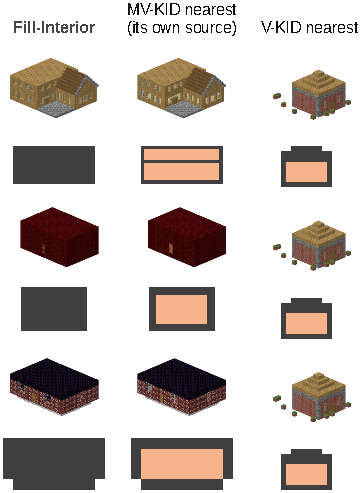
\includegraphics[width=\linewidth]{figures/fig_nn_dissociation}
\caption{\textbf{Each feature space is blind where the other sees.} Three filled 3D-Craft
houses (left), the nearest held-out real build in \mvkid{}'s feature space (middle) and in
\vkid{}'s (right), each over a cross-section with sealed air in peach. The render features
return the house's own source for every one of $256$ filled houses; \vkid{}'s features
return it for $26\%$ (median source rank $17.5$) and send a filled house to a few dense
hub builds, the same one for all three rows. For \matshuffle{} the pattern reverses:
\vkid{} returns the source every time and the render features $26\%$. For held-out real
builds the two spaces pick the same nearest reference build $3.9\%$ of the time (chance
$0.25\%$).}
\label{fig:nn}
\end{figure}

\begin{figure*}[t]
\centering
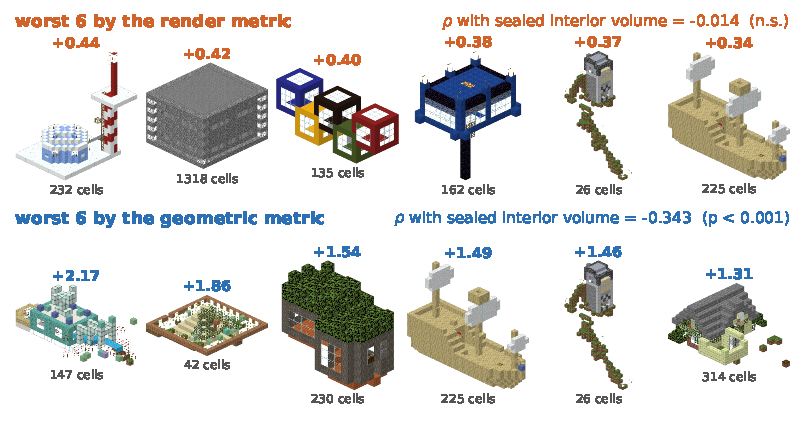
\includegraphics[width=\linewidth]{figures/fig11_influence}
\caption{\textbf{The two metrics disagree about real builds, with no probe involved.} The
unbiased estimator is a sum over builds, so each build's contribution to its arm's score is
recoverable. The six builds each metric penalizes most are shown with their contribution and
their sealed interior volume. The two orderings are nearly independent, $\rho = +0.167$, and
only the geometric ordering tracks how much interior a build has: its rank correlation with
sealed interior volume is $-0.343$ ($p < 0.001$) against $-0.014$ for the render metric.
Builds shown are 3D-Craft only, for licensing.}
\label{fig:influence}
\end{figure*}

% =====================================================================
\section{LEGO and BrickGPT}
\label{app:brickgpt}
% =====================================================================

BrickGPT \citep{pun2025brickgpt} is trained on the StableText2Brick (ST2B) training split,
so the paper's pooled LEGO corpus is not a fair reference for it. We build the reference
from the $4{,}785$ ST2B \emph{test} structures alone, with no void filter; ST2B test objects
share no object with its training split. The suite's group split divides them
$3{,}349/718/718$ and the reference is $512$ of the $718$ validation structures. We prompt
with one caption of each of $256$ structures drawn from the suite's test partition, so the
prompted objects are in neither the reference nor BrickGPT's training data. Generation uses
the released configuration with three forced deviations: bf16 weights, a mirror of the base
model with identical size, and the repository's documented connectivity rollback in place
of the physics rollback, because the free Gurobi licence refuses every ST2B structure. A
$1{,}800$\,s cap per prompt (not in BrickGPT) produced $3$ failures. Stability is solved
with SCIP on BrickGPT's own formulation, validated against the Gurobi scores ST2B ships
($240$ of $240$ agree, mean difference $4.6\times10^{-7}$).

\begin{table}[h]
\centering
\small
\setlength{\tabcolsep}{3pt}
\caption{BrickGPT's own metrics. Stability is over structures the solver finished.}
\label{tab:brickgpt-validity}
\resizebox{\linewidth}{!}{%
\begin{tabular}{lrrrr}
\toprule
 & valid & stable & mean stab. & min stab. \\
\midrule
paper, physics rollback & $100\%$ & $98.8\%$ & $0.996$ & $0.915$ \\
paper, no rollback & $100\%$ & $24.0\%$ & $0.947$ & $0.228$ \\
\textbf{ours, connectivity rollback} & $\mathbf{98.8\%}$ & $\mathbf{95.8\%}$ & $\mathbf{0.995}$ & $\mathbf{0.896}$ \\
held-out real (same $256$) & $100\%$ & $100\%$ & $0.997$ & $0.953$ \\
\bottomrule
\end{tabular}}
\end{table}

Table~\ref{tab:brickgpt-validity} places our run close to the published full method. The
three-point stability gap is what replacing the physics rollback by the
connectivity rollback should cost, since a connected but cantilevered structure passes the
connectivity check. On the suite ($n{=}253$, $77$-dimensional descriptor), BrickGPT sits at
$+11.77$ on appearance and $+51.48$ on geometry, \blockscore{} $51.48$, behind the
solidified control at $36.41$ ($-0.09$ appearance), and the held-out structures matched to
its prompts score like real ($0.40$). Its largest-component ratio is $0.980$ against $0.999$
and its sealed interior $0.011$ against $0.034$, so part of its geometric gap is interior
volume the render tier cannot see. It is not disqualified on novelty.
Fig.~\ref{fig:lego} shows the domain in its own colors.

\begin{figure*}[t]
\centering
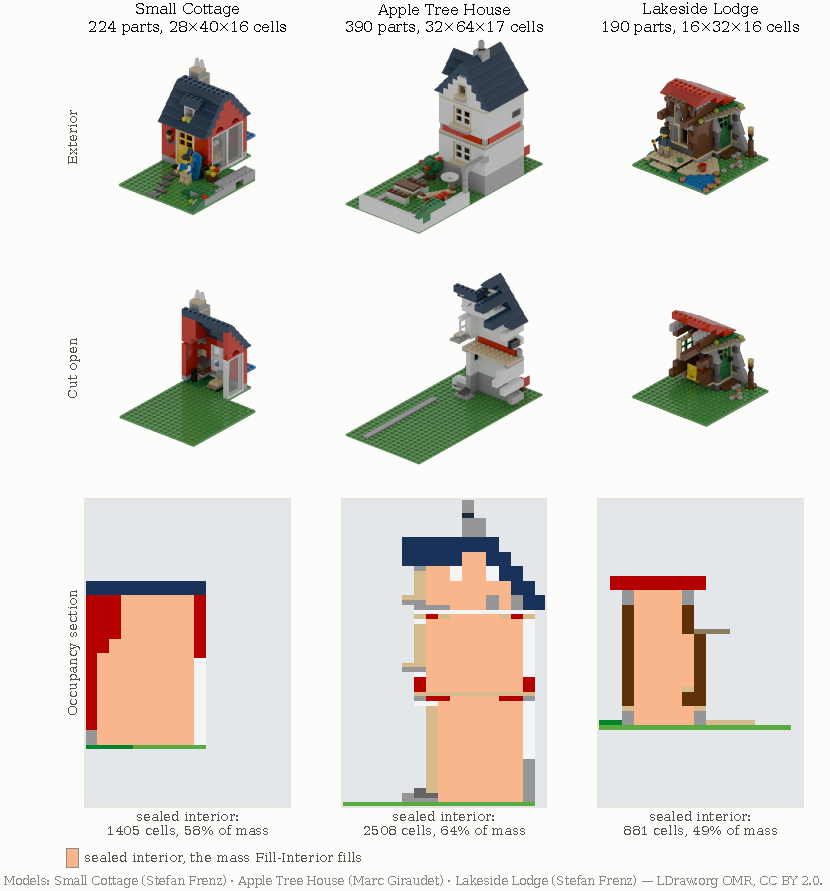
\includegraphics[width=0.72\linewidth]{figures/fig8_lego_omr}
\caption{\textbf{A second domain, with real colors.} Three LDraw.org OMR models in their
own LEGO colors: the exterior an exterior protocol sees, the same parts cut past one
plane, and the occupancy grid we derive sliced at that plane, sealed interior in peach,
every other color the parts' own, all renders at one scale. This domain shares only the
fact that builds enclose space: different parts, different lattice, different renderer, $190$--$390$ parts against
thousands of blocks. The measured replication of
\mainsec{sec:lego} runs on StableText2Brick rather than on these three models, which we
picture because their terms permit it (Sec.~\ref{app:data}). Official LEGO sets are
far less hollow than either measured corpus: among models with at least eight sealed cells,
the basis the OMR audit reports, \solidify{} adds a median $+1.2\%$ mass to an OMR model
against $+35.8\%$ to a held-out house. Models: Small Cottage (Stefan Frenz), Apple Tree House (Marc Giraudet), Lakeside
Lodge (Stefan Frenz); LDraw.org OMR, CC BY 2.0, modified only by the deletions shown.}
\label{fig:lego}
\end{figure*}

% =====================================================================
\section{Leaderboard Arms and Real Generators}
\label{app:leaderboard}
% =====================================================================

This section documents the one external submission, the contamination case study
and the blindness on $40$ real generators. Fig.~\ref{fig:samples} shows six builds of
every leaderboard arm.

\subsection{Dream-Cubed}
\label{app:dreamcubed}

Dream-Cubed \citep{merino2026dreamcubed} is a $279$M-parameter 3D diffusion transformer
over $32^3$ Minecraft chunks, conditioned on one of $15$ biome classes and trained on
procedurally generated worlds that contain no GrabCraft, 3D-Craft or text2mc build. We run
the \texttt{MD4\_p4\_boosted} checkpoint (Apache-2.0), conditioned on \texttt{village},
with the configuration's own classifier-free guidance of $4.0$ and $1{,}000$ reverse steps,
for $288$ chunks; the leaderboard scores the first $256$ extracted builds.

\paragraph{Extraction rule.} A sample is a village on terrain. We keep the constructed
blocks; count sandstone only where no terrain block lies above it in its column, since
desert sub-surface is sandstone under sand; select the $26$-connected component with the
most non-log blocks, so a bare tree never wins; crop it to its bounding box; and drop chunks
whose component has fewer than $80$ blocks. \textbf{$284$ of $288$ chunks yield a build.}
The rule is ours and favours the model, so the whole chunk is scored beside it as a control:
every chunk is a $32$-wide slab of stone and dirt, and the diversity gate disqualifies it
for mode collapse at $+24.0$ spreads. Two vocabulary losses come from Dream-Cubed itself:
its slab and stair tokens carry no material (mapped to stone slab and oak stairs), and its
block names carry no variants (planks, logs and wool map to their first variant). Both
raise its palette pillar, which reads $+87.65$ and never determines its \blockscore{}.

\paragraph{Novelty against the training split.} Against the houses\_32 training split the
extracted builds reach a mean nearest-neighbor voxel IoU of $0.42$, against $0.38$ for
held-out real, and one of $256$ ($0.004$) is a duplicate at IoU $0.95$, against $0.008$ for
held-out real. That gate compares against our training split only.

\paragraph{Within-set near-twins, and the gate they prompted.} The builds repeat one
another. For each build we take its nearest other build in the same set, at the best
occupancy IoU over the $8$ yaw and mirror variants and every integer translation (exact,
by FFT cross-correlation). $59.8\%$ of Dream-Cubed's $256$ builds have such a twin at IoU
$\geq 0.8$, against $0.8\%$ of held-out real, and the median nearest-twin IoU is $0.85$
against $0.42$. The largest group among all $284$ extracted builds holds $28$ copies of
one $117$-block hut. Size does not explain it: restricted to Dream-Cubed's block-count
interquartile range and matched at $98$ builds per set, the rate is $73\%$ against $0\%$.
Neither existing gate sees this. The duplicate gate compares to the training split, and
the diversity gate averages over all pairs, which $160$ clusters of near-copies still
pass ($0.866$ against $0.898$ for real). We therefore added a third novelty gate, the
\emph{within-set near-twin rate}, under the same rule as the duplicate gate: an arm is
disqualified when its rate lies more than $3$ spreads above the real control of the same
run, with a spread of at least $0.02$. At $n{=}256$ the bar is $0.068$. Fresh real draws
of $256$ sit well below it ($0.006$, $0.008$ and $0.019$ on average from the test,
validation and training splits). The gate judges submissions, not diagnostics: probes
that rewrite real builds are exempt, since filling interiors makes real houses genuinely
more alike ($0.066$ for \solidify{}), while the repeated-build control stays judged.
Every model we trained reads $0.000$. The gate
disqualifies Dream-Cubed at $+29.5$ spreads, and with it the two parametric baselines,
\hollowbox{} ($0.246$) and \gabled{} ($0.207$), whose shapes repeat with different
materials. It reads occupancy only.

\paragraph{What the builds are, and the templates control.} Of the $284$ extracted
builds, $45\%$ are houses with a room, $36\%$ are roofless enclosures and $19\%$ are
fragments, against $99\%$ houses in held-out real, at a median of $272$ blocks against
$675$ for the reference. Size carries at most $7\%$ of the geometric distance:
refitting the standardizer without the $\log(1+n_{\text{blocks}})$ column moves raw
\vkid{} from $7.67$ to $7.17$, and scoring against only the $111$ reference builds inside
Dream-Cubed's own block-count interquartile range ($155$--$462$) raises it to $8.57$. Their
median best IoU to the $299$ village templates of the current game version is $0.52$,
against $0.32$ for held-out real, and none reaches $0.9$. As a control, we pass the current
templates through Dream-Cubed's own extraction and score them under the leaderboard's
protocol: $174$ house templates survive the $80$-block floor ($183$ village templates in
all). Their pillars would give a \blockscore{} of $202.95$ ($194.98$ for all $183$),
geometry-limited, ahead of every model we trained, from a set that involves no learning.
They repeat each other as well ($67.2\%$ twins), and the near-twin gate disqualifies them
at $+33.2$ spreads. Scored in the same run, Dream-Cubed reproduces its leaderboard values
exactly.

\subsection{Case study: contamination no statistic sees}
\label{app:casestudy}

%TL;DR of paragraph: the case study asks whether the suite catches a failure we did not build, and a required provenance declaration finds it in three arms where every distribution statistic reads clean.
The main results use corruptions we built, where ground truth is known by construction.
This case study asks whether the suite catches a failure we did not build. A generator we
control is the right subject, because its training split is knowable. The suite requires
every arm to declare that split. \voxar{}, the top-ranked submission of the protocol run,
declared one that contained $346$ of the $399$ canonical test builds ($87\%$). \llmft{} and
\llmgeo{} declared an earlier $90/10$ shuffle holding $53$ of the $399$ ($13\%$). No
distribution statistic sees either. In the protocol run, \voxar{}'s duplicate rate is $0.000$ and its retrieval
percentile $0.509$ against a real held-out floor of $0.534$, far from the verbatim-copy
control at $+10.7$ spreads ($+10.1$ on the $n{=}256$ leaderboard).

%TL;DR of paragraph: retraining on the clean split erases the margin and turns the cross-track result into a tie, and the gate disqualifies the sibling checkpoint.
Retraining \voxar{} on the canonical split, with architecture and hyperparameters
unchanged, isolates the effect (Fig.~\ref{fig:contamination}). We report raw \vkid{},
the statistic the permutation test of Sec.~\ref{app:significance} compares; all four
arms were scored together in the protocol run at $n{=}128$, against one reference. Contaminated, the arm
scores $11.62$ and separates from one language-model baseline at Holm
$5.5{\times}10^{-3}$; clean, it scores $14.898$ against their $15.006$ and $15.869$ and
separates from neither. Under a correctly calibrated test it never held a significance group
alone (Table~\ref{tab:casestudy}). Contamination lowers an arm's distance from real,
so the baselines' own contamination flatters them and we report that comparison as not
separated. The sibling \voxarun{}, retrained on the same clean split at a duplicate rate of
exactly $0.000$, sits on the memorization bar: at $n{=}128$ its retrieval percentile of
$0.382$ against a real floor of $0.534$ is $+3.0$ spreads, which the gate disqualifies, and at
$n{=}256$ it reads $0.403$ against $0.507$, $+2.1$ spreads, and ranks fourth. A gate decision
this close to its bar is a question of sample size, which is why the protocol asks for
$n \geq 256$.

\paragraph{The language-model arms.} \llmft{} and \llmgeo{} appear only in the
protocol run's case study, not on the leaderboard. They decode at temperature
$0.8$ under a $1{,}200$-token cap, and that cap limits both arms: $11$ of $128$
generations came back empty, $139$ attempts were needed for $128$ samples, and
several completions are truncated into structures one block thick.

%TL;DR of paragraph: a required field beats every detector.
What detected both contaminations was a required field rather than a detector: every
memorization gate passed and the declaration did not, so benchmarks in this domain should
require that declaration and refuse to rank arms that cannot make it.

\begin{table}[t]
\centering
\small
\caption{Retraining on a clean split collapses the margin. \vkid{} at
$n{=}128$ (protocol run), $399$-build reference, paired and Holm-corrected over all $120$ pairs
with an exact label-permutation test. Letters mark maximal sets of arms that no
test separated at $\alpha=0.05$: a shared letter means the pair was \emph{not
separated}, never that the arms are equivalent, and an arm carries several
letters when non-separation fails to be transitive, as it does here. The
contaminated arm is not separated from either its own clean retrain or the
stronger language-model baseline, and the clean retrain ties with both baselines
it had appeared to beat. \voxarun{}'s memorization gate is marginal here ($+3.0$
spreads against a bar of $3.0$) and does not fire at $n{=}256$
(Sec.~\ref{app:n256}).}
\label{tab:casestudy}
\setlength{\tabcolsep}{3pt}
\resizebox{\linewidth}{!}{%
\begin{tabular}{llrcl}
\toprule
& arm & \vkid{} $\downarrow$ & group & status \\
\midrule
& \realheld{} (floor)      & $-0.095$ & a & --- \\
& \traincopy{}         & $0.960$  & b & DQ memorization \\
\midrule
\multirow{5}{*}{\rotatebox{90}{\footnotesize submissions}}
& \voxar{}$^{\dagger}$ \emph{(contaminated)} & $11.624$ & \textbf{c} & unranked \\
& \textbf{\voxar{}} \emph{(clean)} & $14.898$ & \textbf{cd} & ranked \\
& \llmft{}            & $15.006$ & \textbf{cd} & ranked \\
& \llmgeo{}               & $15.869$ & \textbf{d} & ranked \\
& \voxarun{} \emph{(clean)} & $19.570$ & e & \textbf{DQ memorization} \\
\midrule
& \patchstitch{}               & $19.976$ & e & ranked \\
& \randomvox{}         & $37.729$ & h & ranked \\
\bottomrule
\end{tabular}}
\end{table}

\begin{figure*}[t]
\centering
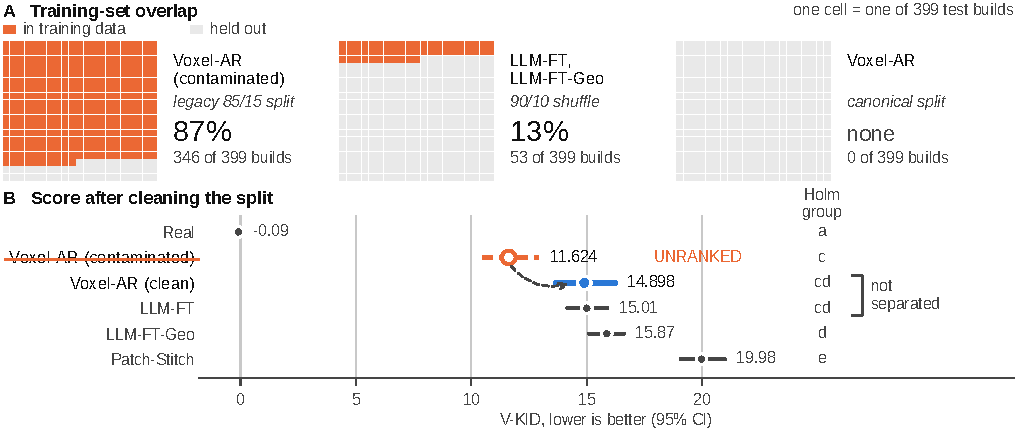
\includegraphics[width=0.90\linewidth]{figures/fig_contamination}
\caption{\textbf{Declared provenance, and what it cost.} \emph{A:} how much of the
canonical test split each arm had already trained on; the third waffle is \voxar{}
retrained on that split. \emph{B:} the retrain costs $+3.27$ raw \vkid{} and erases the
margin. No memorization gate fires on the contaminated arm, so it is unranked rather than
disqualified.}
\label{fig:contamination}
\end{figure*}

% =====================================================================
% rankflips.tex: replaces \subsection{The blindness on real generators}
% (\label{app:rankflips}) in sec/X_appendix.tex, from that \subsection line
% through the end of the fig:rankflips float (\label{fig:rankflips} ...
% \end{figure*}). The fig:samples float that follows it in the file is NOT part
% of this replacement; leave it where it is.
% Labels defined here: app:rankflips, tab:rankflips, fig:rankflips (kept),
% app:functional, tab:functional (new).
% Sources: outputs/run_20261108_205428_stats_fixes/rankflips_exact.json (pairs,
% rho), outputs/run_20261109_152704_rankflips_functional_rebase/results.json
% (functional split on the 40 pairs, 34 decisions under the exact test, worked
% examples), outputs/run_20261108_204723_functional_groundtruth/results.json (FD),
% outputs/run_20261106_193513_render_blind_rank_flips/results.md (hidden blocks,
% ceiling, hollowed outputs).
% =====================================================================
\subsection{The blindness on real generators}
\label{app:rankflips}

The probes of the main text alter real builds. This section asks whether the same blindness
changes conclusions about generators. We pool every house generator scored against the
$399$-build validation reference at the protocol's $n$ under the current renderer: $22$
autoregressive voxel models (scale, temperature, best-of-$k$, rejection fine-tuning,
tokenizer and schedule variants), $10$ facade generators, which emit the six face images of
a build and lift them into the voxel grid, $5$ LLM program generators, the two clean 3D-BPE
models of the leaderboard and BrickNet \citep{kulits2026bricknet}, $40$ in all, $35$ of them
at $n{=}256$ and the LLM arms at $n{=}128$ to $133$. Both metrics are recomputed from the
per-build features of every arm, matched to its card by hash (\mvkid{} to $3\times10^{-6}$).
Every pair is tested with the exact label-permutation test of Sec.~\ref{app:significance}
against the fixed reference, $20{,}000$ permutations, Holm-corrected over all $780$ pairs per
metric. The test stays exact at unequal sizes, and the $35$ arms at $n{=}256$ are also
reported alone. The interval on $\rho$ half-samples every arm and the reference jointly.

\begin{table}[h]
\centering
\small
\setlength{\tabcolsep}{4pt}
\caption{\textbf{Agreement of the two rankings over real generators.} Spearman correlation
of the \mvkid{} and \vkid{} orderings with a half-sampling $95\%$ interval. Pairs: separated
by both metrics under the exact permutation test after Holm correction over all $780$, and
the subset the two metrics order oppositely.}
\label{tab:rankflips}
\resizebox{\linewidth}{!}{%
\begin{tabular}{lrccc}
\toprule
generators & $k$ & $\rho$ & both sep. & opposite \\
\midrule
all & $40$ & $0.50$ \scriptsize{$[0.37, 0.58]$} & $308$ & $\mathbf{40}$ \\
at $n{=}256$ & $35$ & $0.60$ \scriptsize{$[0.46, 0.67]$} & $255$ & $24$ \\
autoregressive voxel & $24$ & $0.37$ \scriptsize{$[0.16, 0.51]$} & $58$ & $7$ \\
facade & $10$ & $0.99$ \scriptsize{$[0.88, 1.00]$} & $32$ & $0$ \\
\bottomrule
\end{tabular}}
\end{table}

\paragraph{Where the rankings part.} The interval of Table~\ref{tab:rankflips} reflects
sampling of builds. Resampling the generators themselves widens it to $[0.20, 0.72]$, and a
cluster bootstrap over the five families to $[0.02, 0.91]$: the correlation is a property of
this pool's family mix. Without the facade family it is $0.28$; without the voxel family,
$0.72$. In $22$ of the $40$ reversed pairs the render metric prefers a facade generator.
Facade generators emit shells: a median $0.5\%$ of their blocks have no face on exterior air,
against $15.6\%$ for held-out houses and $12.5\%$ for the voxel models, and moving from the
\mvkid{} to the \vkid{} ranking costs the family $7.7$ places on average. Across all $40$
generators, however, the shift between the two rankings correlates with the share of hidden
blocks only at $\rho{=}-0.26$ ($p{=}0.10$), so hidden mass alone does not explain the
reordering. The pair of Fig.~\ref{fig:rankflips} is tied under \mvkid{}, $3.1$ noise floors
apart (Holm $p{=}1$), and $292.9$ floors apart under \vkid{} (Holm $p{=}0.039$, the smallest
value $20{,}000$ permutations can reach over $780$ pairs); with the roof removed, the facade
builds are walls around an empty floor. Next to the same voxel model, a best-of-four facade
generator is preferred by \mvkid{} by $55.1$ floors and rejected by \vkid{} by $209.5$, both
at the same Holm floor.

\paragraph{The ceiling of a shell generator.} Reducing each held-out house to the cells its
six faces show gives the output of a perfect facade generator. It sits $8.1$ noise floors
from real data under \mvkid{}, ahead of every trained generator by more than $90$ floors,
and at $+310.6$ under \vkid{}, $19$th of $41$. Applied to generator output, \hollow{}
deletes the blocks no camera sees from our best voxel model, $15\%$ of its mass, and moves
it from $5$th to $29$th of $41$ under \vkid{} ($+147.5$ floors). On the same $128$ builds,
rendered and scored together with their hollowed copies, \mvkid{} moves $+0.15$ noise floors
and \vkid{} $+117.1$; for the 3D-BPE model the two read $+0.18$ and $+139.2$. The converse
holds as well: a voxel model sampled at temperature $0.7$ is over-solid, $24\%$ hidden
blocks, and hollowing its output moves it $24.7$ floors \emph{closer} to real data under
\vkid{}. \vkid{} therefore sees what is deleted from a generator's interior; whether what it
sees is damage is a separate question, which Sec.~\ref{app:functional} answers.

\paragraph{Design decisions.} We list $34$ decisions taken while building these generators,
each a pair of arms that differ in one choice (temperature, best-of-$k$, rejection
fine-tuning, scale, D4 augmentation, tokenizer, schedule, LLM loop), and test each with the
same exact permutation test, Holm-corrected over the $34$. The two metrics agree on $6$ and
never disagree in sign when both are significant; $13$ are significant under neither. On
$15$ the verdict depends on the pillar: $14$ are significant under \mvkid{} alone, among them
D4 augmentation of the 20M facade model ($-52.4$ floors under \mvkid{}, $+16.9$ under
\vkid{}), and $1$ under \vkid{} alone, replacing voxels with 3D-BPE pieces ($+162.6$ floors
worse under \vkid{}, $+21.5$ under \mvkid{}). Most decisions that change a score change
what the exterior shows; local geometry moves beyond noise in $7$ of the $34$.

\paragraph{Scope.} The $40$ generators come from one project. \vkid{} is a distribution
distance on local geometry, not a counter of hidden blocks: the LLM program arms are also
near-shells and move up, not down, under \vkid{}, and the best facade generator has the
lowest \vkid{} of the pool, below its own ceiling, because sampling at temperature $0.7$
narrows its size and shape distribution toward the reference mode. Under the
$80$-dimensional descriptor of the current cards, $29$ of the $308$ both-separated pairs
reverse and the correlation rises to $0.65$ $[0.54, 0.71]$; every statement above holds.

\begin{figure*}[t]
\centering
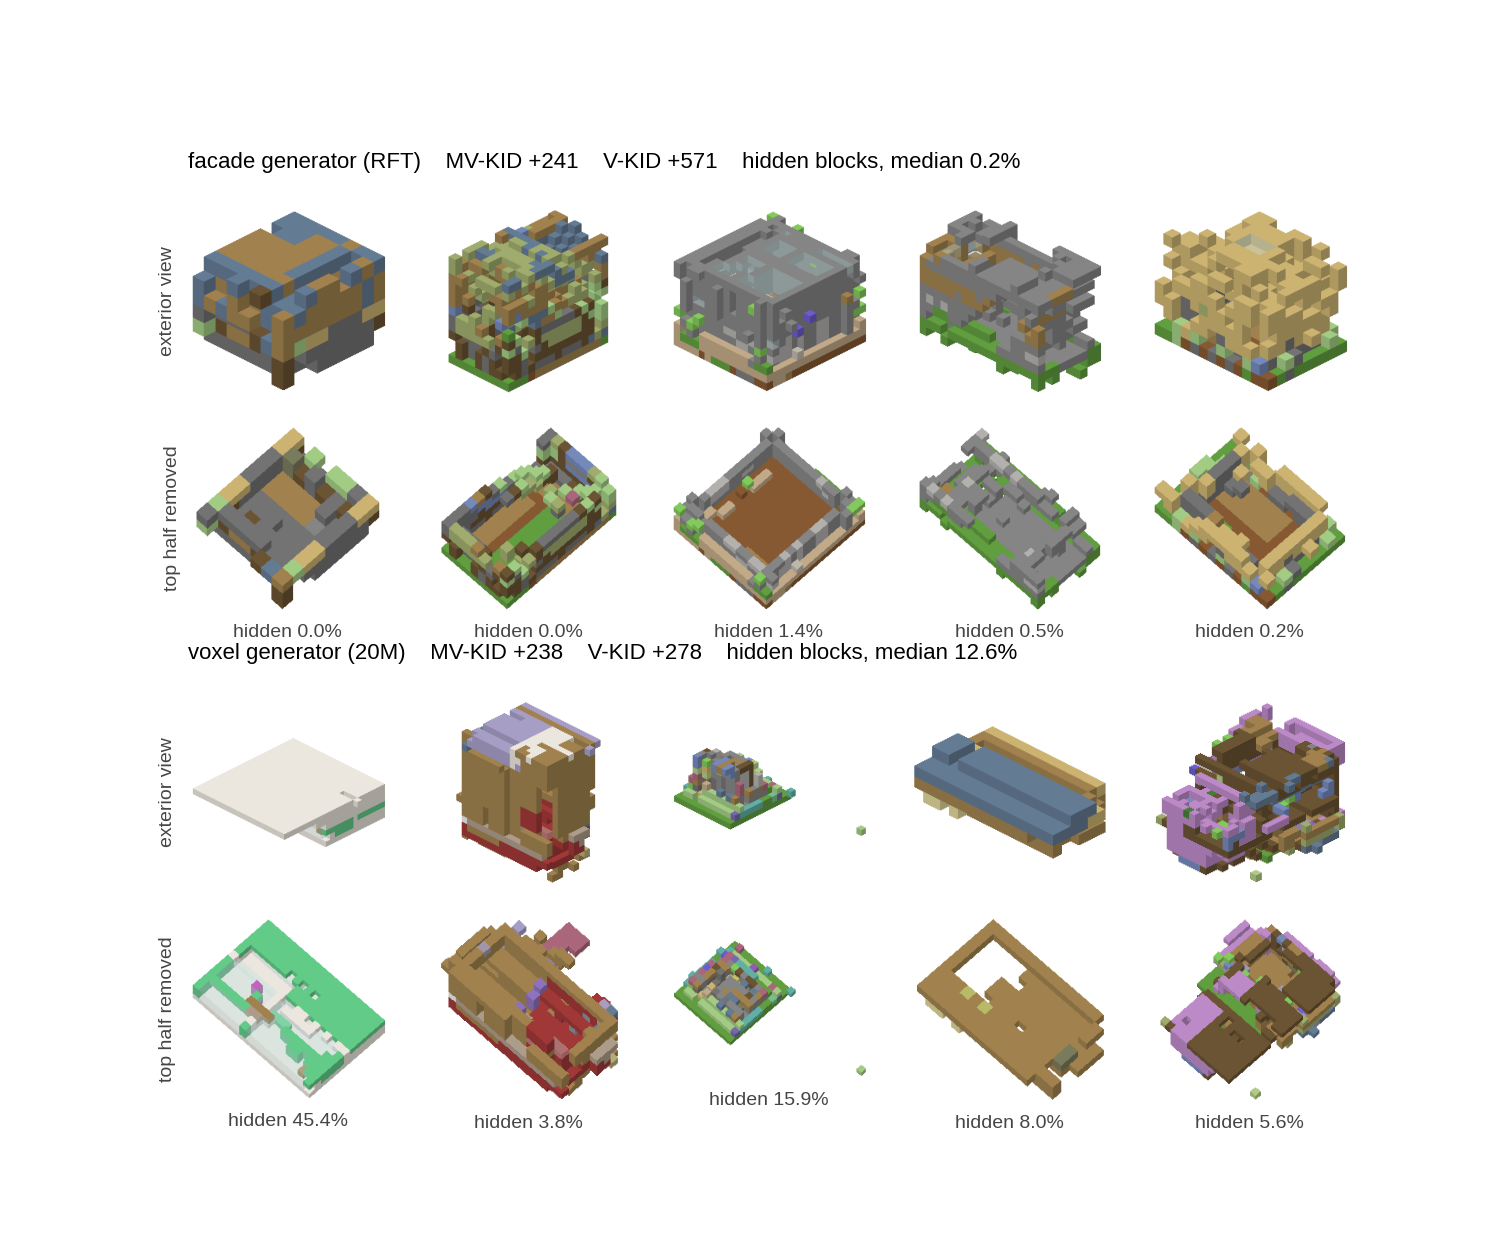
\includegraphics[width=0.8\linewidth]{figures/rankflips_samples}
\caption{\textbf{Tied under \mvkid{}, $293$ floors apart under \vkid{}.} The first five
builds of each arm that pass the memorization gate, generated output only. Top of each block:
the exterior corner view of the protocol; bottom: the same build with its upper half
removed. The facade generator's builds are walls around an empty floor, a median $0.2\%$ of
blocks hidden from every exterior ray; the voxel model's hold partitions and fill, $12.6\%$
($15.6\%$ for held-out houses).}
\label{fig:rankflips}
\end{figure*}

\subsection{Detection is not ranking: a functional ground truth}
\label{app:functional}

The probes establish that \vkid{} detects a change to a real interior that \mvkid{} cannot
see. On the $40$ reversed pairs the question is different: which ranking orders generators
by how usable their interiors are. We answer it with a test that reads neither metric's
features.

\paragraph{A walk-through test.} Every build is set on flat ground and entered by the player
of the traversability probe, a body two blocks tall that steps up one block, falls, climbs
ladders and opens doors. Five measures follow: whether the player reaches any interior
standing cell (\emph{enterable}); how many interior standing cells it reaches (\emph{floor});
how many rooms it reaches, a room being a component of interior air holding at least six
standing cells, with doorways closed so that a doorway separates two rooms; whether at least
half of the plan is roofed by a block with two free cells beneath it; and the share of blocks
in the largest 6-connected component. Held-out houses average $0.94$, $80$ cells, $1.36$
rooms, $0.81$ and $0.98$. \vkid{} has no reachability, door semantics, room labelling, plan
shelter or component analysis; a cross-validated ridge regression on its $77$ features
explains $R^2 = 0.29$ to $0.62$ of the per-build measures. The functional distance FD of an
arm is the mean over the five measures of the Wasserstein-1 distance to the validation
reference, each in units of the real between-build spread, with $1{,}000$ bootstrap
replicates that share one reference resample. Three variants check the construction: units
of real-versus-real sampling distance at $n{=}256$, a cubic-kernel KID on the standardized
measures, and an occupancy-only version without door semantics.

\paragraph{The test sees interiors.} Held-out real data ranks first of $41$ under all four
variants, at FD $0.09$ $[0.08, 0.19]$ against $0.52$ for the best generator. \solidify{}
reaches $1.21$, cutting the enterable share from $0.94$ to $0.20$, and \hollow{} $0.60$:
the walk-through detects the two probes \mvkid{} cannot, so its verdict on generators is not
a second exterior observer.

\paragraph{On generators it follows the render ranking.} Over the $40$ generators, FD
correlates with \mvkid{} at Spearman $0.67$ $[0.41, 0.82]$ and with \vkid{} at $0.16$
$[-0.20, 0.45]$, with intervals that resample generators and FD replicates jointly. The
maximum of the two, which \blockscore{} reads, correlates at $0.17$ $[-0.18, 0.45]$, because
geometry is the worse pillar for $37$ of the $40$. On the $40$ reversed pairs, every FD
difference is significant, and the walk-through sides with \mvkid{} in $33$ and with \vkid{}
in $7$ ($18\%$, Clopper--Pearson $[7, 33]$). The facade family does not produce this. On the
$18$ pairs without a facade generator it sides with \vkid{} in none ($[0, 19]\%$); on the
$22$ facade pairs it does so in $7$, five of them BrickNet preferred over a facade generator,
and BrickNet's builds are almost never enterable ($0.8\%$). The variants agree ($2$, $9$ and
$8$ of $40$ for the noise-unit, KID and occupancy-only distances; none of the $18$
non-facade pairs under the occupancy-only one), and leaving out any one generator keeps the
share between $6\%$ and $24\%$. Taken one measure at a time, enterability, reached floor and
reached rooms side with \vkid{} on none of the $40$.

\paragraph{Why.} The autoregressive voxel generators do not emit shells; they clutter their
interiors. A median $22\%$ of their builds can be entered, against $94\%$ of held-out houses,
with a median $3.4$ reachable floor cells against $80$. Their walls, block patterns and
sealed air have the local statistics of real houses, and \vkid{} scores those statistics.
Deleting the hidden blocks of the best voxel model moves it $147.5$ \vkid{} floors away from
real data and $0.41$ functional units toward it ($1.32$ to $0.90$), and the one design
decision \vkid{} alone flags, 3D-BPE pieces over voxels, is one the walk-through prefers
($1.34$ against $1.67$). Detection of interior change is not ranking of interior function.
The probes hold, since \solidify{} and \hollow{} are functional damage on real houses that
renders cannot see. On current generators, though, the dominant interior failure co-varies
with defects the render tier sees, and a local volumetric descriptor reads it as realism. A
leaderboard that ranks by interior function needs a functional pillar beside both tiers.

\begin{table}[h]
\centering
\small
\setlength{\tabcolsep}{3pt}
\caption{\textbf{Functional ground truth.} Top: functional distance to real (FD, $95\%$
bootstrap interval) and enterable share. Bottom: on the $40$ pairs the two metrics order
oppositely, how often the walk-through agrees with each, and its Spearman correlation with
each ranking over the $40$ generators.}
\label{tab:functional}
\resizebox{\linewidth}{!}{%
\begin{tabular}{lcc}
\toprule
arm & FD & enterable \\
\midrule
held-out real & $0.09$ \scriptsize{$[0.08, 0.19]$} & $0.95$ \\
\solidify{} & $1.21$ \scriptsize{$[1.11, 1.32]$} & $0.20$ \\
\hollow{} & $0.60$ \scriptsize{$[0.52, 0.73]$} & $0.95$ \\
best generator (LLM program) & $0.52$ \scriptsize{$[0.43, 0.65]$} & $0.68$ \\
best voxel model under \vkid{} & $1.32$ \scriptsize{$[1.20, 1.43]$} & $0.28$ \\
\quad same, hidden blocks deleted & $0.90$ \scriptsize{$[0.78, 1.04]$} & $0.59$ \\
\midrule
 & with \mvkid{} & with \vkid{} \\
reversed pairs, all $40$ & $33$ & $7$ \\
reversed pairs, $18$ without a facade arm & $18$ & $0$ \\
reversed pairs, $22$ with a facade arm & $15$ & $7$ \\
Spearman over $40$ generators & $0.67$ \scriptsize{$[0.41, 0.82]$} & $0.16$ \scriptsize{$[-0.20, 0.45]$} \\
\bottomrule
\end{tabular}}
\end{table}


\begin{figure*}[p]
\centering
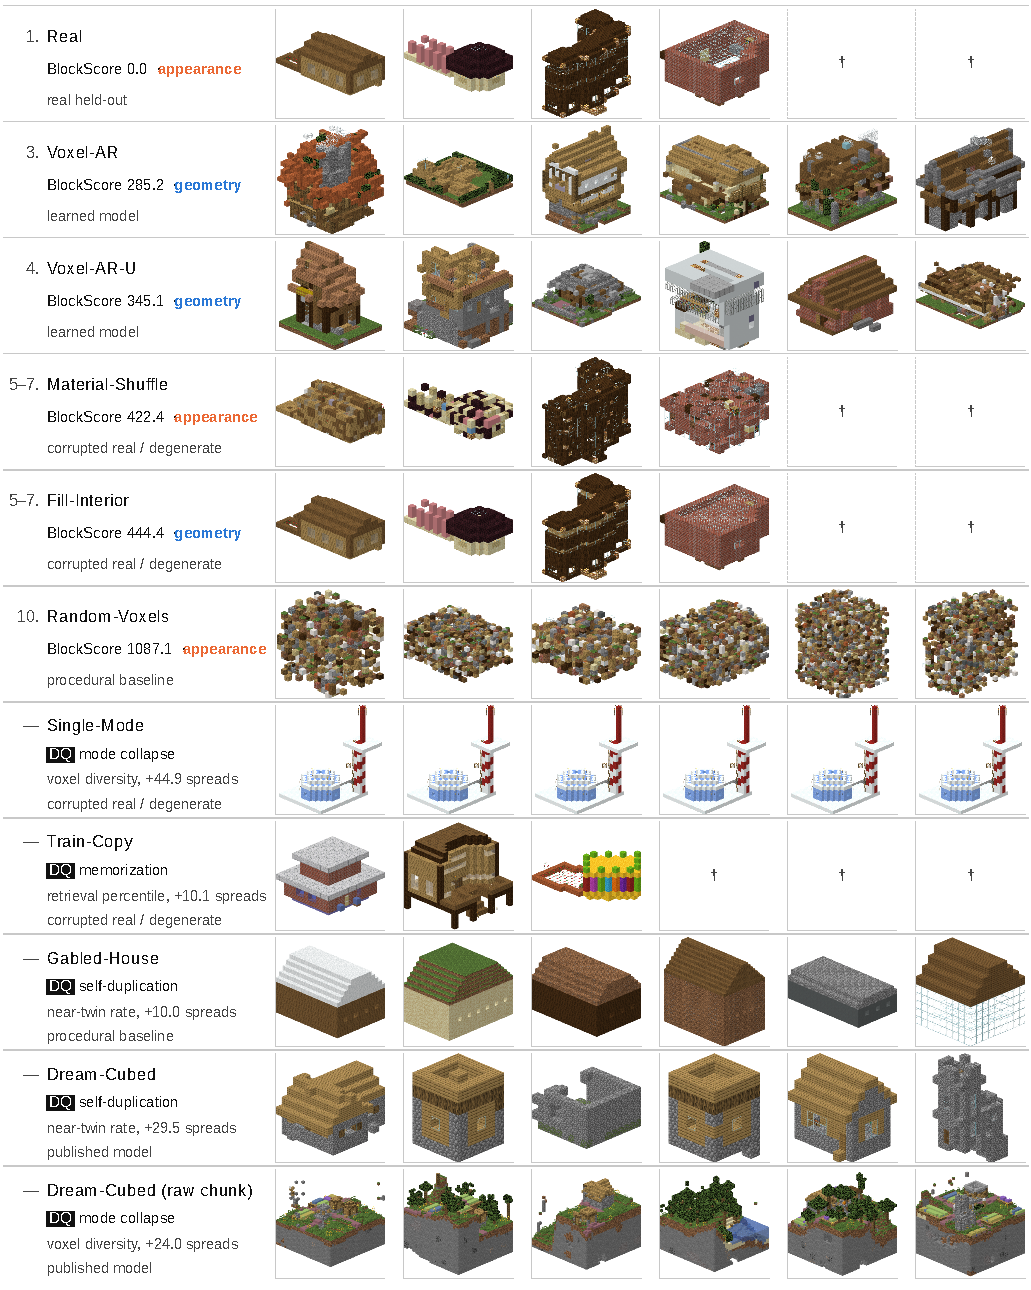
\includegraphics[width=\linewidth]{figures/fig_samples}
\caption{\textbf{Every arm, ordered by \blockscore{}} ($n{=}256$ leaderboard). Six builds
per arm: the first six the run recorded, in the seeded order it recorded them, topped up from
that arm's full scored sample where fewer than six remain. \realheld{}, \solidify{} and
\matshuffle{} are the same buildings column for column, so a corruption reads down a column
and the paper's central claim can be checked by eye: the \solidify{} row scores $+444.36$ on
geometry and $+0.35$ on appearance. Cells marked $\dagger$ are withheld under GrabCraft's
terms, so the real-derived rows show four builds. Dream-Cubed is the extracted arm
(Sec.~\ref{app:dreamcubed}); its whole-chunk control is the last row. Each build is
framed to its own bounding box, so cells are not to a common scale, and \texttt{DQ} marks
an arm a disqualification gate refused a rank (\maintab{tab:leaderboard}). No generated
build shown is a memorized copy: none of the $48$ generated cells reaches IoU $0.95$ to a
training build. The contaminated checkpoint of Fig.~\ref{fig:contamination} is absent: it
is unrankable, and a gallery ordered by score would imply a standing it does not have.}
\label{fig:samples}
\end{figure*}

% =====================================================================
\section{Reproducibility, Data and Licences}
\label{app:data}
% =====================================================================

\paragraph{Released artifacts.} The evaluation suite, the probes, the procedural
baselines and the group-aware split are released and contain no upstream content.
Every benchmark run writes a scorecard recording corpus, split hash, $n$,
reference size, seed, host, device and commit, so each number in the paper is
traceable to the run that produced it; the release README lists the runs of
record and their cache manifests. \TODO{Add the anonymized code URL and commit,
and the institutional determination covering the corpus release, before
submission.}

\paragraph{Compute.} Every run in the paper uses one workstation: one NVIDIA
GeForce RTX 5070 Ti ($16$\,GB), a $12$-core AMD Ryzen 9 9900X and $32$\,GB of RAM.
The $n{=}256$ leaderboard, rendering and embedding every arm and running the
ladder and the head-to-head tests, takes $1{,}115$\,s end to end, and the
$n{=}128$ protocol run $411$\,s. \vkid{} alone takes $15$ to $18$\,s on one CPU
process (Sec.~\ref{app:headtohead}). Training \voxar{} takes about two hours on
the same GPU.

\paragraph{Corpus and redistribution.} Our Minecraft corpus derives from three
public sources: the 3D-Craft house dataset \citep{chen2019voxelcnn,gray2019craftassist},
released with the CraftAssist project; a scrape of \texttt{grabcraft.com}; and the
text2mc dump, whose builds originate from \texttt{planetminecraft.com}. \textbf{We
do not redistribute the GrabCraft- or text2mc-derived structures.} GrabCraft's
terms permit sharing blueprints only by linking, and PlanetMinecraft's terms
prohibit redistributing site data. We release instead the curation code, the
per-build source URLs, content hashes, the group-aware split as index lists, and
a rebuild script, so the corpus reproduces bit-exactly without our distributing
third-party content. Builds are credited by source URL in the released
manifests; the original scrape did not capture uploader names.

\paragraph{Licences.} The 3D-Craft house data ships without a licence file and
its distributing release, \texttt{facebookresearch/voxelcnn}, is CC BY-NC 4.0, so
we treat it as non-commercial research material requiring attribution, not under
the CraftAssist code's MIT terms. StableText2Brick and the BrickGPT code and
weights are MIT-licensed; the dataset derives from ShapeNetCore, whose terms
restrict use to non-commercial research. Dream-Cubed's village checkpoint and its
data repository are Apache-2.0; we run its code for evaluation and do not
redistribute it. The LDraw.org OMR models of Fig.~\ref{fig:lego} are CC BY 2.0.

\paragraph{Depiction.} Every real build shown in this paper comes from
\textbf{3D-Craft only}, since GrabCraft's terms name pictures of blueprints as a
prohibited form of distribution; generated builds are shown as generated. Figures
render builds with Minecraft's own texture assets, which are Mojang's copyright and
which Mojang's usage guidelines permit in non-commercial images. The release
contains \textbf{no texture files}, so a reader reproducing our figures supplies
them from their own installation, and the figure scripts also produce flat
per-block colors that need no permission. Minecraft features: \copyright{} Mojang
Synergies AB, included courtesy of Mojang AB. This is not an official Minecraft
product and is not approved by or associated with Mojang or Microsoft.


{
    \small
    \bibliographystyle{ieeenat_fullname}
    \bibliography{references,references_new}
}

\end{document}
